% ============================================================================
% BracU thesis project assembled from the user's Thesis_Template.zip,
% Thesis P2.docx / main (1).tex, and Chapter4_Methodology_IEEE_Overleaf.zip.
% Overleaf: upload this whole ZIP. Compiler: pdfLaTeX. Bibliography tool: Biber.
% ============================================================================
\documentclass[12pt,oneside,openany]{report}
\usepackage[a4paper,width=150mm,top=25mm,bottom=25mm]{geometry}
\usepackage[english]{babel}
\usepackage[T1]{fontenc}
\usepackage[utf8]{inputenc}
\usepackage{newunicodechar}
\newunicodechar{ć}{\'{c}}
\usepackage{textcomp}
\usepackage{csquotes}
\usepackage{amsmath,amssymb}
\usepackage{graphicx}
\graphicspath{{images/}{figures/}}
\usepackage{caption}
\usepackage{array,booktabs,longtable,multirow,tabularx,makecell,calc}
\newcounter{none}
\usepackage{xcolor}
\usepackage{url}
\usepackage{algorithm}
\usepackage[noend]{algpseudocode}
\usepackage{tikz}
\usetikzlibrary{positioning,arrows.meta,shapes.geometric,shapes.misc,fit,calc,backgrounds,decorations.pathreplacing}
\usepackage{pgfplots}
\pgfplotsset{compat=1.18}
\usepackage{adjustbox}
\usepackage{etoolbox}
\usepackage[nottoc]{tocbibind}
\usepackage{hyperref}
\hypersetup{colorlinks=true,linkcolor=black,filecolor=magenta,urlcolor=black,citecolor=black}
\urlstyle{same}
\setlength{\parindent}{0em}
\setlength{\parskip}{0.35em}
\setlength{\emergencystretch}{3em}
\let\cleardoublepage=\clearpage

% Pandoc's Word-to-LaTeX export marked source text with \hl; here it is deliberately
% neutralized so the thesis text is not yellow-highlighted.
\long\def\hl#1{#1}
\providecommand{\tightlist}{\setlength{\itemsep}{0pt}\setlength{\parskip}{0pt}}

% Chapter 4 helper commands/styles carried over from the supplied IEEE project.
\definecolor{navy}{HTML}{1E4E8C}
\definecolor{navylt}{HTML}{EEF3FA}
\definecolor{amber}{HTML}{C0701A}
\definecolor{amberlt}{HTML}{FFF3E3}
\definecolor{teal}{HTML}{16877F}
\definecolor{teallt}{HTML}{E6F4F2}
\definecolor{greyd}{HTML}{8C929B}
\definecolor{greylt}{HTML}{F2F3F5}
\definecolor{ink}{HTML}{1B2330}
\definecolor{redlt}{HTML}{FDECEC}
\definecolor{redd}{HTML}{B42318}
\newcommand{\cond}[1]{\texttt{\small #1}}
\newcommand{\condt}[1]{{\ttfamily\scriptsize #1}}
\newcommand{\tl}[1]{\textit{#1}}
\newcolumntype{Y}{>{\raggedright\arraybackslash}X}
\newcolumntype{L}[1]{>{\raggedright\arraybackslash}p{#1}}
\newcolumntype{H}[1]{>{\raggedright\arraybackslash\hspace{0pt}}p{#1}}% ragged, first word may hyphenate
\renewcommand{\arraystretch}{1.1}
\tikzset{
  box/.style={draw=navy, rounded corners=2pt, align=center, fill=navylt, font=\scriptsize, inner sep=3pt, line width=0.6pt},
  lora/.style={box, fill=navy, text=white, draw=navy},
  safe/.style={box, fill=amberlt, draw=amber},
  cpu/.style={box, fill=teallt, draw=teal},
  grey/.style={box, fill=greylt, draw=greyd},
  arr/.style={-{Stealth[length=1.8mm]}, line width=0.7pt, draw=ink},
  darr/.style={arr, dashed},
  lab/.style={font=\tiny, align=center, text=ink},
}
\pgfplotsset{every axis/.append style={font=\scriptsize, tick label style={font=\tiny}, label style={font=\scriptsize},
    legend style={font=\tiny, draw=none, fill=none}, axis line style={draw=greyd}, tick style={draw=greyd},
    ymajorgrids, grid style={draw=greylt}, axis x line*=bottom, axis y line*=left,
    legend image code/.code={\fill[#1] (0cm,-0.07cm) rectangle (0.28cm,0.07cm);}}}
% Scale only over-wide TikZ diagrams to the BracU thesis text width.
\BeforeBeginEnvironment{tikzpicture}{\begin{adjustbox}{max width=\textwidth}}
\AfterEndEnvironment{tikzpicture}{\end{adjustbox}}

\usepackage[backend=biber,style=ieee,sorting=ynt]{biblatex}
\addbibresource{bibliography/references.bib}
\AtBeginBibliography{\setlength{\emergencystretch}{10em}}

\begin{document}
\thispagestyle{empty}
\begin{titlepage}
\renewcommand*{\thepage}{Title}
\begin{center}
\vspace*{2.2cm}
{\fontsize{16pt}{21pt}\selectfont{Bridging Bangla Dialects and Standard Bangla:\\[3pt]
A Dialect-Aware Bangla Question Answering with\\
Routed Domain Experts and Retrieval-Augmented\\
Generation for Healthcare and Education}}

\vspace{1.3cm}
by

\vspace{0.55cm}
MD. Nafiul Haque Nafee\\23101244\\[0.25cm]
Tausif Ishrak\\23101007\\[0.25cm]
Kaspia Khan Onti\\23101145\\[0.25cm]
Saleha Sattar Oishy\\23101045

\vspace{1.35cm}
A thesis submitted to the Department of Computer Science and Engineering\\
in partial fulfillment of the requirements for the degree of\\
B.Sc. in Computer Science and Engineering

\vfill
Department of Computer Science and Engineering\\
Brac University\\
October 2026

\vspace{1.1cm}
\copyright\ 2026. Brac University\\
All rights reserved.
\end{center}
\end{titlepage}

\cleardoublepage

\pagenumbering{roman}
\phantomsection\addcontentsline{toc}{chapter}{Declaration}\section*{Declaration}

It is hereby declared that

\begin{enumerate}
  \item The thesis submitted is our own original work while completing our degree at Brac University.

  \item The thesis does not contain material previously published or written by a third party, except where this is appropriately cited through full and accurate referencing.

  \item The thesis does not contain material which has been accepted, or submitted, for any other degree or diploma at a university or other institution.

  \item We have acknowledged all main sources of help.
\end{enumerate}

\vspace{1.2cm}

\textbf{Student's Full Name \& Signature:}

\vspace{0.35cm}

\begin{center}

\begin{tabular}{c@{\hspace{1.4cm}}c}

% =========================================================
% Row 1: MD. Nafiul Haque Nafee and Tausif Ishrak
% =========================================================

\makebox[6.2cm][c]{%
  
\includegraphics[
    width=5.9cm,
    height=2.4cm,
    keepaspectratio,
  ]{figures/signature_nafee.jpg}
}
&
\makebox[5.4cm][c]{%
  
\includegraphics[
    width=4.2cm,
    height=1.15cm,
    keepaspectratio
  ]{figures/signature_tausif.png}
}
\\

\rule{6.2cm}{0.4pt}
&
\rule{5.4cm}{0.4pt}
\\

MD. Nafiul Haque Nafee
&
Tausif Ishrak
\\

23101244
&
23101007
\\[0.9cm]


% =========================================================
% Row 2: Kaspia Khan Onti and Saleha Sattar Oishy
% =========================================================

\makebox[6.2cm][c]{%
  
\includegraphics[
    width=4.0cm,
    height=1.15cm,
    keepaspectratio
  ]{figures/signature_kaspia.png}
}
&
\makebox[5.4cm][c]{%
  
\includegraphics[
    width=4.3cm,
    height=1.15cm,
    keepaspectratio
  ]{figures/signature_saleha.jpg}
}
\\

\rule{6.2cm}{0.4pt}
&
\rule{5.4cm}{0.4pt}
\\

Kaspia Khan Onti
&
Saleha Sattar Oishy
\\

23101145
&
23101045

\end{tabular}

\end{center}

\clearpage
\phantomsection\addcontentsline{toc}{chapter}{Approval}\section*{Approval}

The thesis titled ``Bridging Bangla Dialects and Standard Bangla: A Dialect-Aware Bangla Question Answering with Routed Domain Experts and Retrieval-Augmented Generation for Healthcare and Education'' submitted by

\begin{enumerate}
    \item MD. Nafiul Haque Nafee (23101244)
    \item Tausif Ishrak (23101007)
    \item Kaspia Khan Onti (23101145)
    \item Saleha Sattar Oishy (23101045)
\end{enumerate}

of Fall, 2026 has been accepted as satisfactory in partial fulfillment of the requirement for the degree of B.Sc. in Computer Science and Engineering on [date of defense].

\vspace{0.5cm}

\textbf{Examining Committee:}

\vspace{0.5cm}

% =========================================================
% Supervisor
% =========================================================

\noindent
\begin{minipage}[t]{0.33\textwidth}\raggedright
    \textbf{Supervisor:}\\
\end{minipage}
\hfill
\begin{minipage}[t]{0.62\textwidth}
    \centering

    \vspace{1.0cm}

    \rule{6.5cm}{0.4pt}\\
    \textbf{Dr. Md. Khalilur Rahman}\\
    Professor\\
    Department of Computer Science and Engineering\\
    Brac University
\end{minipage}

\vspace{0.8cm}


% =========================================================
% Thesis Coordinator
% =========================================================

\noindent
\begin{minipage}[t]{0.33\textwidth}\raggedright
    \textbf{Thesis Coordinator:}\\
\end{minipage}
\hfill
\begin{minipage}[t]{0.62\textwidth}
    \centering

    \vspace{1.0cm}

    \rule{6.5cm}{0.4pt}\\
    \textbf{Dr. Md. Golam Rabiul Alam}\\
    Professor\\
    Department of Computer Science and Engineering\\
    Brac University
\end{minipage}

\vspace{0.8cm}


% =========================================================
% Head of Department
% =========================================================

\noindent
\begin{minipage}[t]{0.33\textwidth}\raggedright
    \textbf{Head of Department:}\\
\end{minipage}
\hfill
\begin{minipage}[t]{0.62\textwidth}
    \centering

    \vspace{1.0cm}

    \rule{6.5cm}{0.4pt}\\
    \textbf{Sadia Hamid Kazi, PhD}\\
    Associate Professor and Chairperson\\
    Department of Computer Science and Engineering\\
    Brac University
\end{minipage}

\clearpage
\phantomsection\addcontentsline{toc}{chapter}{Abstract}\section*{Abstract}
There are many Bangla speakers who communicate using regional variations such as Sylhet and Chittagonian. While existing Bangla question answering systems and language models are developed and evaluated on Standard Bangla, this creates a particular gap in the Healthcare sector and education sector in the domain where reliable information is important. This study proposes a dialect aware multi domain Bangla QA framework based on router driven mixture of expert architecture. These frameworks collect questions in Bangla dialect or standard Bangla and responses according to that input. A light weight routing model first recognises standard Bangla and linguistic variety of the input and its domain. These inputs and questions are then normalized into standard Bangla if it is recognized by the model as a dialect before being routed to the proper domain so that each domain is supported by a dedicated retrieval augmented generation (RAG) pipeline so that it matches the response generation in relevant external evidence. There will be multiple predetermined language models where the framework compares several open source Bangla adapted TigerLLM and other suitable architectures. These models are adapted using efficient fine tuning methods such as LoRA and QLoRA. The framework is determined using Bangla question answering and domain specific resources including NCTB-QA, BanglaRQA and BanglaCHQ. The evaluation covers dialect identification and normalization, retrieval effectiveness, end-to-end QA performance, clarification and abstention behavior. Then the results are separately reported across that specific dialect language or standard Bangla with component wise studies and comparisons across candidate base models. This study aims to reduce the performance disparity between standard Bangla and dialect users by developing a modular retrieval, grounded and domain hour QA framework that provides standard Bangla responses while being computationally practical for low resource Bangla NLP.

\vspace{0.5cm}
\textbf{Keywords:} Bangla NLP, Bengali medical chatbot, Bengali educational chatbot, Chittagonian, Sylheti, dialect normalization, dialect routing, question answering, retrieval-augmented generation, medical safety, Gemma 4, TigerLLM, LoRA, QLoRA, mixture of adapters, NCTB-QA, BanglaRQA, BanglaCHQ, low-resource NLP
\clearpage

\phantomsection\addcontentsline{toc}{chapter}{Acknowledgement}\section*{Acknowledgement}

We would like to express our sincere gratitude to our thesis supervisor,
\textbf{Dr. Md. Khalilur Rahman}, for his continuous guidance, constructive
feedback, encouragement, and support throughout this work.

We also extend our appreciation to the authors and contributors of the public
datasets, models, tools, and research resources on which this work builds.
Their contributions made it possible to conduct the experiments and evaluations
presented in this thesis.

We are also grateful to the faculty members and the Department of Computer
Science and Engineering at Brac University for providing an encouraging
academic and research environment throughout the development of this thesis.

Finally, we would like to thank everyone who directly or indirectly supported
us during the completion of this work.

\clearpage

\renewcommand{\contentsname}{Table of Contents}
\tableofcontents\clearpage
\listoffigures\clearpage
\listoftables\clearpage
\chapter*{Nomenclature}
\addcontentsline{toc}{chapter}{Nomenclature}
The following abbreviations are used in this thesis.
\begin{longtable}{@{}p{0.22\textwidth}p{0.72\textwidth}@{}}
ASR & Automatic Speech Recognition\\
BLEU & Bilingual Evaluation Understudy\\
BM25 & Best Matching 25 (sparse retrieval function)\\
CER / WER & Character / Word Error Rate\\
chrF / chrF++ & Character n-gram F-score (++: with word n-grams)\\
CI & Confidence Interval\\
Ctg / Syl & Chittagonian / Sylheti\\
DEV / TEST & Validation split / held-out test split\\
ECE & Expected Calibration Error\\
EM & Exact Match\\
KB & Knowledge Base\\
LLM & Large Language Model\\
LoRA & Low-Rank Adaptation\\
MCQ & Multiple-Choice Question\\
MoE & Mixture of Experts\\
MRR & Mean Reciprocal Rank\\
NCTB & National Curriculum and Textbook Board\\
nDCG & Normalized Discounted Cumulative Gain\\
NF4 & 4-bit NormalFloat quantization\\
QA & Question Answering\\
QLoRA & Quantized Low-Rank Adaptation\\
RAG & Retrieval-Augmented Generation\\
RRF & Reciprocal Rank Fusion\\
SVM & Support Vector Machine\\
TF-IDF & Term Frequency--Inverse Document Frequency\\
\end{longtable}
\clearpage


\pagenumbering{arabic}
\chapter{Introduction}
\hl{Bangla is spoken by more than 270 million people \cite{jawad2026fivedialects}, but most
language technology for Bangla understands only one form of it: Standard
Bangla. As with many languages spoken by many people, naturally, there
are many variations to how Bangla is spoken. These variations are
dialects and this creates a communication barrier between people from
different regions. At home and online, many people write the way they
speak, in a regional dialect such as Chittagonian or Sylheti, or type
Bangla with Latin letters (romanized Bangla). This chapter explains why
that matters for question answering (QA) in healthcare and education,
states the problem, the research questions and the objectives,
summarises the method and the contributions, and sets out the scope and
the main challenges of the work.}

\section{Background}\label{background}

\hl{Ranking among the world's most prominent languages by total
speakers, Bangla has a significant global presence; across Bangladesh,
India and the diaspora, millions of people use it as their first or
second language \cite{shafayat2024benqa}, \cite{jawad2026fivedialects}. Bangla has a strong regional dialect
continuum: Bangladesh alone has about 55 regional varieties spread over
its 64 districts \cite{faria2023vashantor}, \cite{samin2024bangladialecto}. These varieties differ from Standard
Bangla (cholito bhasha), the form used in textbooks, news and
administration, in pronunciation, vocabulary, verb morphology and word
order. Many speakers learn a regional variety at home and Standard
Bangla only at school. Chittagonian and Sylheti are two of the most
widely spoken and most divergent varieties: in dialect translation and
dialect identification experiments they are consistently among the
hardest to handle \cite{jawad2026fivedialects}, \cite{faria2023vashantor}, \cite{khandaker2024bridging}, \cite{prantik2025}. In our own data, a
Chittagonian sentence and its Standard translation share only 30\% of
their character trigrams, and a Sylheti sentence 35\% (Chapter 4).}

\hl{Resources for natural language processing (NLP) are unevenly
distributed across the world's languages, and low-resource languages
receive only a small share of data, models and benchmarks \cite{joshi2020state}.
Bangla has gained important resources in recent years: pretrained
encoders and sequence-to-sequence models such as BanglaBERT and BanglaT5
\cite{bhattacharjee2022banglabert}, \cite{bhattacharjee2023banglanlg}, Bangla large language models (LLMs) such as TigerLLM
and TituLLMs \cite{raihan2025tigerllm}, \cite{titulm2025}, and QA benchmarks such as BanglaRQA,
NCTB-QA, BEnQA and SOMAJGYAAN \cite{ekram2022banglarqa}, \cite{nctbqa}, \cite{shafayat2024benqa}, \cite{shifa2025somajgyaan}. All
of these, and the textbooks, news articles, encyclopedia passages and
exam papers they are built from, are in Standard Bangla, and models are
evaluated only on Standard Bangla \cite{jawad2026fivedialects}. Figure~\ref{fig:ch1-landscape} summarises this
situation.}

% ---------------- Figure 1.1 (Background) ----------------
\begin{figure}[!htbp]
\centering
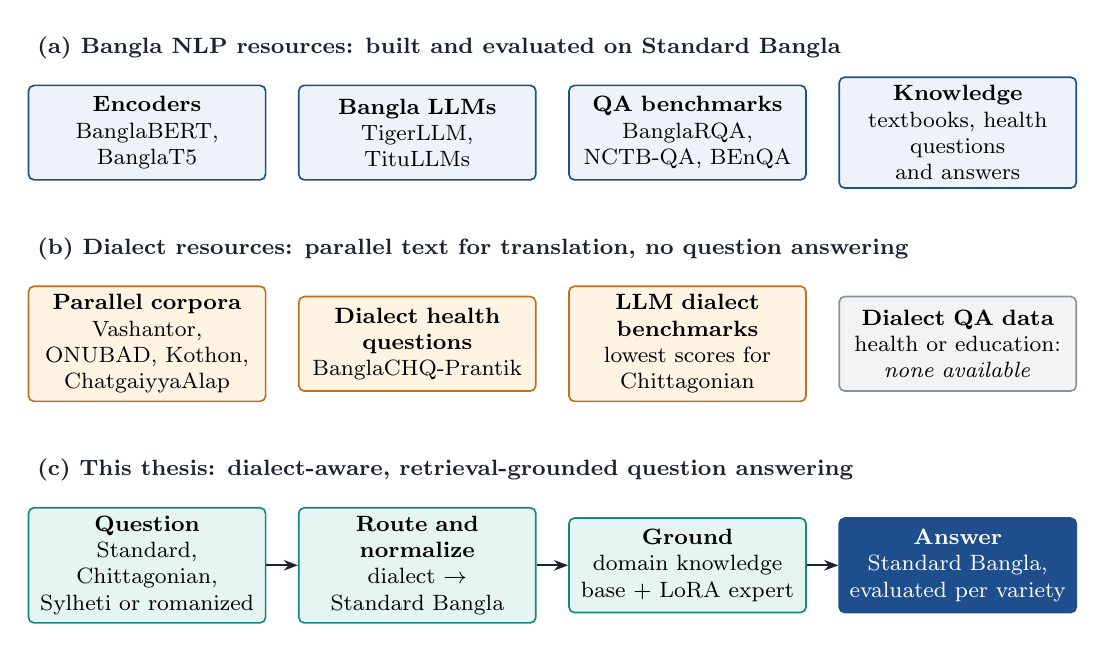
\begin{tikzpicture}[node distance=3mm and 4mm,
  res/.style={font=\footnotesize, text width=28mm, minimum height=12mm, execute at begin node={\hyphenpenalty=10000}},
  hdr/.style={font=\footnotesize\bfseries, text=ink, anchor=west}]
\node[hdr] (h1) at (0,0) {(a) Bangla NLP resources: built and evaluated on Standard Bangla};
\node[box, res, below=2mm of h1.south west, anchor=north west] (r1a) {\textbf{Encoders}\\BanglaBERT,\\BanglaT5};
\node[box, res, right=of r1a] (r1b) {\textbf{Bangla LLMs}\\TigerLLM,\\TituLLMs};
\node[box, res, right=of r1b] (r1c) {\textbf{QA benchmarks}\\BanglaRQA, NCTB-QA, BEnQA};
\node[box, res, right=of r1c] (r1d) {\textbf{Knowledge}\\textbooks, health\\questions and answers};
\node[hdr, below=6mm of r1a.south west, anchor=north west] (h2) {(b) Dialect resources: parallel text for translation, no question answering};
\node[safe, res, below=2mm of h2.south west, anchor=north west] (r2a) {\textbf{Parallel corpora}\\Vashantor, ONUBAD, Kothon, ChatgaiyyaAlap};
\node[safe, res, right=of r2a] (r2b) {\textbf{Dialect health questions}\\BanglaCHQ-Prantik};
\node[safe, res, right=of r2b] (r2c) {\textbf{LLM dialect benchmarks}\\lowest scores for Chittagonian};
\node[grey, res, right=of r2c] (r2d) {\textbf{Dialect QA data}\\health or education:\\\textit{none available}};
\node[hdr, below=6mm of r2a.south west, anchor=north west] (h3) {(c) This thesis: dialect-aware, retrieval-grounded question answering};
\node[cpu, res, below=2mm of h3.south west, anchor=north west] (r3a) {\textbf{Question}\\Standard, Chittagonian, Sylheti or romanized};
\node[cpu, res, right=of r3a] (r3b) {\textbf{Route and normalize}\\dialect $\rightarrow$ Standard Bangla};
\node[cpu, res, right=of r3b] (r3c) {\textbf{Ground}\\domain knowledge base + LoRA expert};
\node[lora, res, right=of r3c] (r3d) {\textbf{Answer}\\Standard Bangla, evaluated per variety};
\foreach \a/\b in {r3a/r3b,r3b/r3c,r3c/r3d}{\draw[arr] (\a) -- (\b);}
\end{tikzpicture}
\caption[Bangla NLP resources, dialect resources and the gap addressed by this thesis.]{(a) Bangla language technology is built on Standard Bangla, while (b) dialect resources support translation but not question answering. (c) This thesis connects the two: dialect questions are normalized into Standard Bangla so that existing Standard-Bangla QA data and knowledge sources can be reused.}
\label{fig:ch1-landscape}
\end{figure}

\hl{Large language models have made open-ended question answering widely
accessible, but they can produce fluent answers that no evidence
supports, a behaviour known as hallucination \cite{ji2023survey}.
Retrieval-augmented generation (RAG) reduces this risk by retrieving
relevant documents at answer time and conditioning the generator on them
\cite{lewis2020rag}. Parameter-efficient fine-tuning with low-rank adaptation
(LoRA) and its quantized variant QLoRA makes it possible to adapt
billion-parameter models on a single GPU \cite{hu2022lora}, \cite{dettmers2023qlora}. The idea of
dividing a task among specialised sub-models chosen by a gating or
routing function goes back to the mixture-of-experts (MoE) literature
\cite{jacobs1991adaptive}, \cite{shazeer2017moe}. Together, these techniques make a modular, grounded
and affordable QA system realistic for a low-resource language.}

\hl{The dialect problem matters most where reliable information is
scarce. In \textbf{healthcare}, Bangladesh has about 9.9 doctors, nurses
and midwives per 10,000 people, and only about 11\% of doctors and
nurses work in rural areas, where about two thirds of the population
live \cite{nuruzzaman2022informing}. Digital health tools mostly serve European users and
languages, and a Bangladeshi triage application reported that a general
speech-to-text service struggled with dialect speech \cite{nahar2025amardoctor}. Real consumer
health questions in Bangla are informal, loosely described and
code-mixed with English medical terms \cite{khan2023nervous}, Bangla telemedicine
consultations are full of vague descriptions, delayed disclosure and
regional expressions, and prioritising patients from such real
consultations is hard even for strong models (best triage macro-F1
0.463) \cite{saha2026doctalkbn}. In \textbf{education}, university students in
Bangladesh already use LLMs for learning \cite{hossain2025ailiteracy}, and
national-curriculum (NCTB) textbooks have become the basis of new Bangla
QA resources and models \cite{raihan2025tigerllm}, \cite{nctbqa}. Yet LLMs answer the same
exam questions less accurately in Bangla than in English \cite{shafayat2024benqa},
earlier Bangla textbook QA systems were extractive models that only
worked when the correct passage was supplied \cite{khondoker2024unlocking}, and no
educational QA resource contains questions asked in a regional dialect.}

\section{Rationale of the Study}\label{rationale-of-the-study}

\hl{\textbf{The dialect gap is large and prompting alone does not close
it.} A benchmark of 19 LLMs on questions in nine Bengali dialects found
far lower scores for Chittagonian (5.44 out of 10) than for Tangail
(7.68) \cite{sami2026dialectbias}. When LLMs are prompted to convert dialect text into
Standard Bangla, some score below a baseline that simply copies the
input unchanged \cite{jawad2026fivedialects}. In the reverse direction (Standard Bangla to
dialect), the best prompted system on dialect health questions reached a
BLEU of only 23.67 for Sylheti, and Chittagonian scores were generally
lower (14.78 in the same setting) \cite{prantik2025}; without retrieved examples,
LLMs failed almost completely at standard-to-dialect translation (BLEU
5--12) \cite{sami2025comparative}. In our own paired evaluation, the same questions asked
in dialect scored 33\% (Chittagonian) and 43\% (Sylheti) lower than in
Standard Bangla when the system did not normalize them (Chapter 5). If a
system does not understand the question, the quality of its knowledge
base and generator hardly matters.}

\hl{\textbf{Small amounts of targeted supervision help.} LoRA
fine-tuning of open LLMs on only 160 examples per dialect raised
Mistral-7B from 16.2 to 73.6 BLEU on dialect-to-English translation,
above every prompted closed-source model \cite{jawad2026fivedialects}. A lightly adapted
dialect component is therefore a realistic way to close much of the gap
at low cost.}

\hl{\textbf{Normalizing into Standard Bangla reuses existing resources.}
Almost all Bangla QA data, textbooks and health information exist only
in Standard Bangla, and building separate datasets and knowledge bases
for every dialect is not realistic. Rewriting a dialect question into
Standard Bangla first lets the system reuse all of them. There is
supporting evidence for this ``translate into the better-resourced
variety'' strategy: appending an English translation of the question
improved LLM accuracy on BEnQA across all subjects \cite{shafayat2024benqa}, and
dialect-to-Standard translation is the central step of Bangla
speech-standardization pipelines \cite{samin2024bangladialecto}.}

\hl{\textbf{Different domains need different evidence and safety
behaviour.} Health answers must be grounded in reviewed information, and
the system must recognise emergencies and know when to refer the user to
a doctor. Education answers should follow the curriculum, and the system
must recognise questions that its sources cannot answer; NCTB-QA makes
42.75\% of its questions unanswerable for this reason \cite{nctbqa}. Routing
questions to domain-specific pipelines keeps the prompts, knowledge
bases and safety rules of each domain separate and easy to inspect, and
small routers that choose a retrieval strategy per question are an
established idea \cite{jeong2024adaptiverag}. Showing users the passages behind each answer
is a simple way to make the system's reasoning inspectable.}

\hl{\textbf{The system must be affordable.} The institutions that would
benefit most, such as rural clinics, schools and small organisations,
cannot run very large models or pay per-question API fees. A design with
CPU routers, one shared open 4-billion-parameter model and a few small
LoRA adapters can be trained and served on one rented GPU \cite{dettmers2023qlora}. This
approach keeps the system easy enough to build for a student project,
yet lightweight enough for constrained budgets.}

\section{Problem Statement}\label{problem-statement}

\hl{Bangla QA systems and LLMs are developed and evaluated mainly on
Standard Bangla \cite{raihan2025tigerllm}, \cite{ekram2022banglarqa}, \cite{nctbqa}, \cite{shafayat2024benqa}. When a question
is written in Chittagonian or Sylheti, or in romanized Bangla, three
problems arise. First, dialect words, verb forms and spellings may be
misunderstood, and because the question shares few words with Standard
Bangla documents, retrieval may fail as well \cite{jawad2026fivedialects}, \cite{prantik2025}. Second,
without grounding in domain-appropriate evidence, a general model may
answer health and education questions from memory, which risks
hallucinated or unsafe answers \cite{ji2023survey}, \cite{saha2026doctalkbn}. Third, the
performance gap between Standard Bangla users and dialect users is not
measured, because existing benchmarks do not report results by language
variety.}

\hl{Formally, a user question \emph{q} is written in a variety \emph{v}
\ensuremath{\in} \{Standard, Chittagonian, Sylheti\} (in Bangla or Latin script) and
belongs to a domain \emph{d} \ensuremath{\in} \{education, general knowledge, medical,
out-of-scope\}. The system must identify \emph{v} and \emph{d}, produce
a Standard Bangla version of \emph{q} when \emph{v} is a dialect or the
text is romanized, retrieve evidence from the knowledge base of
\emph{d}, and return a Standard Bangla answer grounded in that evidence;
or it must ask for clarification, abstain, or give an emergency referral
when an answer would not be reliable or safe. Answer quality should be
as similar as possible across the three varieties.}

\hl{This thesis answers the following research questions:}

\begin{quote}
\hl{\textbf{RQ1} How accurately, and with how well-calibrated
confidence, can a lightweight router identify the language variety and
the domain of a Bangla question?}

\hl{\textbf{RQ2} How well can a parameter-efficiently fine-tuned model
normalize Chittagonian, Sylheti and romanized questions into Standard
Bangla, and how much of the dialect gap in retrieval and answer quality
does this normalization close?}

\hl{\textbf{RQ3} How much do retrieval, fine-tuned domain experts,
domain routing and the answer/clarify/abstain controller contribute to
answer quality and behaviour, and do routed experts outperform a single
shared adapter?}

\hl{\textbf{RQ4} Which open base model offers the best balance of answer
quality, dialect handling and compute cost under an identical
fine-tuning budget, and does Bangla-specific pre-training help after
fine-tuning?}
\end{quote}

\section{Objectives}\label{objectives}

\hl{The main objective is to design, implement and evaluate a
dialect-aware, multi-domain Bangla QA framework that accepts questions
in Standard Bangla, Chittagonian or Sylheti, in Bangla or Latin script,
and returns grounded Standard Bangla answers for education,
general-knowledge and medical questions. The main deliverables are
trained routing models, a dialect normalization expert, domain-specific
RAG experts, an evaluation suite that reports every result separately
for each language variety, and a reproducible code base. The specific
objectives are:}

\begin{itemize}
\item \hl{to build lightweight, calibrated routers that identify the
language variety and the domain of a question \cite{faria2023vashantor}, \cite{bhattacharjee2022banglabert};}

\item \hl{to train a dialect normalization expert that rewrites
Chittagonian, Sylheti and romanized questions into Standard Bangla with
parameter-efficient fine-tuning \cite{jawad2026fivedialects}, \cite{hu2022lora};}

\item \hl{to build a separate knowledge base and retriever for each domain,
and to adapt one shared open base model to each domain with LoRA/QLoRA
experts \cite{lewis2020rag}, \cite{dettmers2023qlora};}

\item \hl{to decide, for every question, whether to answer, ask for
clarification or abstain, and to handle medical emergencies and
medicine-dose requests with deterministic safety rules and a
doctor-referral note \cite{rajpurkar2018squad2}, \cite{kamath2020selective};}

\item \hl{to compare seven open base models, including Gemma 4 and two
Bangla-adapted models (TigerLLM and TituLM) with their original
versions, under an identical fine-tuning budget \cite{raihan2025tigerllm}, \cite{titulm2025},
\cite{gemma4};}

\item \hl{to evaluate every component and the complete system, using
NCTB-QA, BanglaRQA and dialect resources, with results reported
separately for Standard Bangla, Chittagonian and Sylheti, with
ablations, confidence intervals and significance tests, and to test the
system on dialect questions written by native speakers \cite{nctbqa},
\cite{ekram2022banglarqa}.}
\end{itemize}

\section{Methodology in Brief}\label{methodology-in-brief}

\hl{The framework follows a \emph{route, normalize, then ground} design
(Figure~\ref{fig:pipeline} in Chapter 4). A question first passes rule-based safety
checks for emergencies and dose requests. A calibrated linear classifier
on character and word n-grams identifies the variety; if the question is
Chittagonian or Sylheti with enough confidence, or romanized, a
normalization expert rewrites it into Standard Bangla. A second
classifier chooses the domain, and a controller decides whether to
answer, ask for clarification or abstain. For answerable questions, the
retriever of the chosen domain searches that domain's knowledge base
(BM25 for education and general knowledge, dense BGE-M3 retrieval for
medical questions \cite{robertson2009bm25}, \cite{chen2024bgem3}), and the domain's LoRA expert
writes the answer from the three best passages. All experts are small
adapters on one 4-bit Gemma-4-E4B-it model \cite{gemma4}, a
\emph{Mixture-of-Adapters} \cite{hu2022lora}, \cite{houlsby2019adapters}, \cite{shazeer2017moe}. An output guard
adds a doctor-referral note to medical answers and refuses to give
medicine doses. Figure~\ref{fig:ch1-overview} gives an overview of
this pipeline.}

% ---------------- Figure 1.2 (Methodology in Brief) ----------------
\begin{figure}[!htbp]
\centering
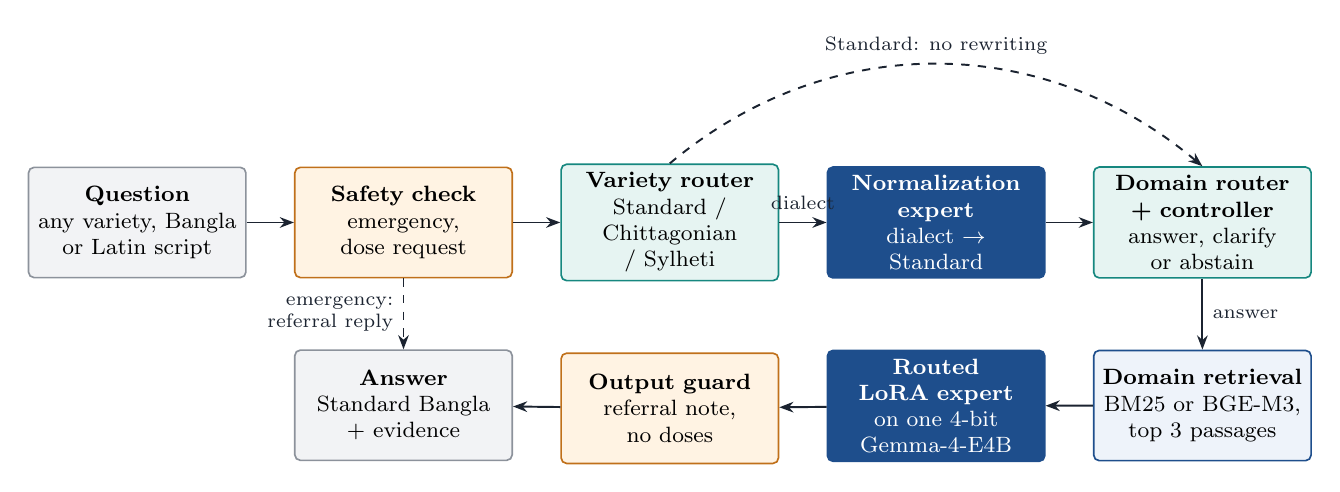
\begin{tikzpicture}[node distance=9mm and 6mm,
  st/.style={font=\footnotesize, text width=25.5mm, minimum height=14mm, execute at begin node={\hyphenpenalty=10000}}]
\node[grey, st] (q) {\textbf{Question}\\any variety, Bangla or Latin script};
\node[safe, st, right=of q] (s) {\textbf{Safety check}\\emergency, dose request};
\node[cpu, st, right=of s] (vr) {\textbf{Variety router}\\Standard / Chittagonian / Sylheti};
\node[lora, st, right=of vr] (n) {\textbf{Normalization expert}\\dialect $\rightarrow$ Standard};
\node[cpu, st, right=of n] (dr) {\textbf{Domain router + controller}\\answer, clarify or abstain};
\draw[arr] (q) -- (s); \draw[arr] (s) -- (vr);
\draw[arr] (vr) -- node[lab, above=1pt, font=\scriptsize]{dialect} (n); \draw[arr] (n) -- (dr);
\draw[darr] (vr.north) to[out=40,in=140] node[lab, above, font=\scriptsize]{Standard: no rewriting} (dr.north);
\node[box, st, below=of dr] (r) {\textbf{Domain retrieval}\\BM25 or BGE-M3, top 3 passages};
\node[lora, st, below=of n] (e) {\textbf{Routed LoRA expert}\\on one 4-bit Gemma-4-E4B};
\node[safe, st, below=of vr] (g) {\textbf{Output guard}\\referral note, no doses};
\node[grey, st, below=of s] (a) {\textbf{Answer}\\Standard Bangla + evidence};
\draw[arr] (dr) -- node[lab, right, font=\scriptsize]{answer} (r);
\draw[arr] (r) -- (e); \draw[arr] (e) -- (g); \draw[arr] (g) -- (a);
\draw[darr] (s) -- node[lab, left, font=\scriptsize, align=right]{emergency:\\referral reply} (a);
\end{tikzpicture}
\caption[Overview of the proposed route, normalize, then ground framework.]{Overview of the proposed \emph{route, normalize, then ground} framework. The routers and the controller run on the CPU; the normalization expert and the domain experts are LoRA adapters on one shared 4-bit model (a Mixture-of-Adapters). Each component is described in Chapter 4 (Figure~\ref{fig:pipeline}).}
\label{fig:ch1-overview}
\end{figure}

\hl{The work was carried out in stages. The data stage cleaned and split
more than twenty public data sources, including four dialect corpora
(Vashantor, Kothon, ChatgaiyyaAlap and ONUBAD), two QA datasets with
unanswerable questions (NCTB-QA and BanglaRQA), textbooks and medical
resources \cite{faria2023vashantor}, \cite{kothon2026}, \cite{chatgaiyyaalap2025}, \cite{sultana2025onubad}, \cite{nctbqa}, \cite{ekram2022banglarqa},
\cite{khan2023nervous}, \cite{aurpa2026banglameder}. Seven open models, including the Bangla-adapted
TigerLLM and TituLM and the multilingual Gemma-4-E4B, Qwen3 and
Llama-3.2, were then compared under an identical QLoRA budget \cite{raihan2025tigerllm},
\cite{titulm2025}, \cite{gemma4}, \cite{qwen3}, \cite{meta2024llama32}, \cite{dettmers2023qlora}. The experts, routers
and retrievers were trained and chosen on validation data, and the test
data were used only once, for reporting. Finally, the complete system
was evaluated under nine conditions on 2,225 paired test questions (780
Standard questions with 720 Chittagonian and 725 Sylheti versions), and
on 481 dialect questions written by native speakers. Every result is
reported separately for each language variety.}

\section{Contributions}\label{contributions}

\begin{enumerate}
\item \hl{\textbf{A modular dialect-aware QA framework} for Bangla that
separates variety routing, dialect normalization, domain routing,
answer/clarify/abstain control, per-domain retrieval, routed LoRA
experts on one shared base model, and medical safety rules, together
with its complete, reproducible implementation.}

\item \hl{\textbf{A fine-tuned dialect normalization expert} for
Chittagonian, Sylheti and romanized input that raises chrF++ from 51.2
to 76.3 (Chittagonian) and from 55.4 to 74.0 (Sylheti) after one epoch
(a second epoch adds 1.3 chrF++ overall), transfers to three dialects
never seen in training, beats similarity-based few-shot prompting, and
on the official Vashantor test sentences equals or exceeds published
dedicated translation models except one (Chittagonian BLEU against
DialectBanglaT5).}

\item \hl{\textbf{A paired, per-variety evaluation protocol} (the same
questions in three varieties, nine system conditions, Holm-corrected
significance tests) that measures the dialect gap end to end. It shows
that normalization closes 61\% (Chittagonian) and 64\% (Sylheti) of the
gap without harming Standard Bangla input; to our knowledge, no earlier
Bangla work measured this downstream effect.}

\item \hl{\textbf{An evaluation on 481 dialect questions written by native
speakers}, which shows that with normalization the system treats a
dialect question like its Standard version 86.1\% of the time (65.3\%
without).}

\item \hl{\textbf{A controlled model comparison and informative negative
results}: under an identical budget, Gemma-4-E4B-it is the best of seven
open models; Bangla continued pre-training gives no advantage after
fine-tuning; routed experts equal a single pooled adapter in accuracy,
so their value is modularity; and a contrastively trained
dialect-invariant retriever is not better overall than its base encoder
and does not reduce the dialect gap.}
\end{enumerate}

\section{Scope and Challenges}\label{scope-and-challenges}

\hl{This thesis builds and evaluates a research prototype, not a
ready-to-use medical product; both its individual parts and the complete
system are evaluated. Its scope and main challenges are listed below.}

\textbf{\hl{Scope of the Study}}

\begin{itemize}
\item \hl{\textbf{Input:} text questions in Standard Bangla, Chittagonian or
Sylheti, written in Bangla script or romanized. Three further dialects
(Barishal, Mymensingh, Noakhali) are used only as unseen test data.
Speech input is not part of this study, although a Bangla medical speech
recogniser with Sylheti recordings \cite{kabir2024asr} could be placed in front of
the system later.}

\item \hl{\textbf{Domains:} education (NCTB curriculum), general knowledge
(Bangla Wikipedia passages of BanglaRQA) and medical questions, each
with its own knowledge base and retrieval pipeline; other questions are
recognised and declined.}

\item \hl{\textbf{Output:} answers in Standard Bangla, with the evidence
shown to the user, because the knowledge sources and most readers use
the standard form. Answering back in the user's dialect is left for
future work.}

\item \hl{\textbf{Healthcare:} general health information only, with
emergency referral and a doctor-referral note; the system does not
diagnose or prescribe.}

\item \hl{\textbf{Compute:} open models trained with QLoRA on one rented
NVIDIA A40 GPU, with all non-GPU work on free Google Colab CPU runtimes
\cite{hu2022lora}, \cite{dettmers2023qlora}.}
\end{itemize}

\textbf{\hl{Key Challenges}}

\begin{itemize}
\item \hl{\textbf{Scarce and uneven dialect data:} Parallel dialect data are
limited and uneven across dialects, and most of them are everyday
conversation rather than health or school questions \cite{faria2023vashantor}, \cite{prantik2025},
\cite{kothon2026}, so domain vocabulary such as symptom names is
under-represented. For example, the medical dialect extension of
BanglaCHQ-Summ contains 2,350 Sylheti but only 500 Chittagonian
questions \cite{prantik2025}.}

\item \hl{\textbf{No standard dialect spelling:} Chittagonian and Sylheti
have no agreed written form, so the same word appears with several
spellings, and romanized text shares almost no words with Bangla-script
text \cite{jawad2026fivedialects}.}

\item \hl{\textbf{No dialect QA test data:} No existing dataset contains
health or education questions in Chittagonian or Sylheti with reference
answers, so the dialect gap has to be measured with generated paired
questions and with human-written dialect questions without reference
answers.}

\item \hl{\textbf{Error propagation:} A wrong variety or domain decision, or
a poor normalization, affects every later stage; the system therefore
uses calibrated confidences and a controller rather than trusting each
component blindly.}

\item \hl{\textbf{Medical safety:} Wrong, overconfident or delayed health
answers can cause harm, and triage is hard even for large models
\cite{saha2026doctalkbn}; emergencies and dose requests must be handled
deterministically.}

\item \hl{\textbf{Unanswerable and vague questions:} Many questions cannot
be answered from the knowledge base or are under-specified; the system
must abstain or ask instead of guessing \cite{rajpurkar2018squad2}, \cite{kamath2020selective}, \cite{nctbqa}.}

\item \hl{\textbf{Evaluating free-text answers:} Medical answers are free
text, and word-overlap metrics under-rate correct answers that use
different words; several metrics, a check of grounding and human review
are needed.}

\item \hl{\textbf{Limited compute and budget:} All training had to fit one
rented GPU and a small budget (about 40 GPU-hours, roughly US\$20),
which makes quantized, parameter-efficient training essential \cite{dettmers2023qlora}.}
\end{itemize}


\chapter{Literature Review}
\hl{The work relevant to this thesis comes from research streams that
have developed largely separately: Bangla dialect processing, Bangla
question answering, Bangla language models, and applications of language
technology in healthcare and education. This chapter first introduces
the concepts the thesis builds on, then reviews the related work,
highlighting its achievements and limitations, and ends with the gaps
that the proposed framework addresses.}

\section{Preliminaries}\label{preliminaries}

\subsection{Bangla and Its Regional Varieties}\label{bangla-and-its-regional-varieties}

\hl{Standard Bangla (cholito bhasha) is the form used in formal writing,
education, broadcasting and administration. The regional varieties form
a continuum across Bangladesh and differ from the standard in
pronunciation, vocabulary, verb morphology and sometimes word order, in
some regions vastly so \cite{jawad2026fivedialects}, \cite{faria2023vashantor}. Chittagonian, spoken in the
south-east, and Sylheti, spoken in the north-east, are among the most
divergent. Online, dialect speakers write in Bangla script with phonetic
spellings of dialect words, or in Latin script (romanized Bangla, often
called Banglish); Sylheti also has a historical script of its own,
Sylheti Nagri \cite{jawad2026fivedialects}. A dialect sentence and its Standard equivalent
can share very few word forms, sometimes none, although they convey
exactly the same meaning, for example Sylheti \emph{kita} for Standard
\emph{ki} (``what''), which is why systems trained on Standard Bangla
misread dialect input.}

\subsection{Dialect Identification and Normalization}\label{dialect-identification-and-normalization}

\hl{Dialect identification predicts the variety a text is written in and
is usually treated as text classification \cite{faria2023vashantor}. Dialect normalization
rewrites a dialect text in the standard variety while keeping its
meaning, which makes it a form of machine translation \cite{faria2023vashantor}, \cite{jawad2026fivedialects}.
Its quality is measured with BLEU \cite{papineni2002bleu}, the character n-gram
F-scores chrF and chrF++ \cite{popovic2015chrf}, \cite{popovic2017chrfpp}, and word or character error
rate (WER, CER). A useful sanity check is the copy-input baseline, which
scores the unchanged dialect input against the Standard reference: a
system that scores below it has made the text worse \cite{jawad2026fivedialects}.}

Both tasks are long-standing problems in NLP for closely related
languages, varieties and dialects \cite{zampieri2020survey}. Dialect identification
is usually framed as supervised text classification, and in shared tasks
for Arabic it has reached high scores: the best systems of NADI 2023
reached a macro-F1 of 87.27 on country-level Arabic dialect
identification \cite{abdulmageed2023nadi}. Normalization is much harder than
identification. In the same shared task, the best systems that
translated Arabic dialects into Modern Standard Arabic reached only
14.76 and 21.10 BLEU on the two machine-translation subtasks
\cite{abdulmageed2023nadi}. Normalization is easier to learn when parallel
dialect--standard data exist, as in the MADAR corpus of 25 city
dialects \cite{bouamor2018madar}, and character-level models suit it because dialect
words are often spelling variants of standard words: for Swiss German,
character-based neural translation was the best normalization strategy
\cite{honnet2018swissgerman}.

Romanized input is a related problem. Bangla written in Latin letters
has no fixed spelling, so the same word appears in many forms, and
converting it back into Bangla script (back-transliteration) is a task
of its own. BanglaTLit provides 42.7k romanized--Bangla-script pairs for
this task, together with a 245.7k-sample romanized pre-training corpus
\cite{fahim2024banglatlit}. In this thesis, romanized questions are
normalized by the same expert that normalizes dialect questions, so
back-transliteration and dialect normalization are handled in one step.

\subsection{Question Answering}\label{question-answering}

\hl{In extractive QA the answer is a span of a given passage, scored
with exact match (EM) and token-level F1 \cite{ekram2022banglarqa}; in multiple-choice QA
the system picks an option and is scored by accuracy \cite{shafayat2024benqa}, \cite{shifa2025somajgyaan};
in open-domain QA the system must first find the evidence itself,
usually with a retriever followed by a reader \cite{karpukhin2020dpr}. When the answer
is generated in the system's own words, evaluation relies on semantic
similarity measures such as BERTScore \cite{zhang2020bertscore} and on checking whether
the generated answer is supported by the evidence \cite{es2024ragas}. A realistic
system must also recognise questions it cannot answer. SQuAD 2.0 added
more than 50,000 unanswerable questions written adversarially by crowd
workers to look answerable, and showed that models trained only on
answerable questions answer them confidently \cite{rajpurkar2018squad2}. Selective QA
trains a calibrator that lets a model abstain when it is unsure, trading
coverage for accuracy \cite{kamath2020selective}.}

\hl{Most of the early Bangla QA systems follow the reading-comprehension
setting, where the passage is given for context and answer searching. A
practical system must instead first retrieve relevant documents from a
knowledge base with a retriever and then pass the top-k documents to a
reader model, which is the retriever--reader design of open-domain QA
\cite{karpukhin2020dpr}. The framework in this research follows that design, with an
LLM as the reader.}

\subsection{Large Language Models and Parameter-Efficient Fine-Tuning}\label{large-language-models-and-parameter-efficient-fine-tuning}

\hl{Modern LLMs are Transformers pre-trained on large text collections
and then instruction-tuned. Updating all their parameters is too
expensive for most academic budgets. LoRA freezes each pretrained weight
matrix \emph{W} \ensuremath{\in} \ensuremath{\mathbb{R}}\textsuperscript{d\ensuremath{\times}k} and learns a low-rank update
\ensuremath{\Delta}\emph{W} = \emph{BA} with \emph{B} \ensuremath{\in} \ensuremath{\mathbb{R}}\textsuperscript{d\ensuremath{\times}r}, \emph{A} \ensuremath{\in}
\ensuremath{\mathbb{R}}\textsuperscript{r\ensuremath{\times}k} and \emph{r} \ensuremath{\ll} min(\emph{d}, \emph{k}) \cite{hu2022lora}.
Only \emph{A} and \emph{B} are trained, which reduces the number of
trainable parameters by several orders of magnitude, and different
adapters can be attached to the same base model for different tasks.
QLoRA stores the frozen base model in 4-bit NormalFloat (NF4) precision
with double quantization and paged optimizers and back-propagates
through it into the LoRA adapters, so billion-parameter models can be
fine-tuned on one GPU with little loss in quality \cite{dettmers2023qlora}.}

\subsection{Retrieval-Augmented Generation}\label{retrieval-augmented-generation}

\hl{RAG combines a retriever that finds passages relevant to the
question with a generator that writes the answer from them \cite{lewis2020rag}.
Sparse retrieval such as BM25 scores documents by weighted term overlap
and works well when question and document share words \cite{robertson2009bm25}. Dense
retrieval encodes questions and passages as vectors and ranks by vector
similarity, which also matches paraphrases and synonyms \cite{karpukhin2020dpr};
multilingual embedding models such as multilingual E5 and BGE-M3 support
Bangla \cite{chen2024bgem3}, \cite{wang2024me5}. Hybrid systems fuse sparse and dense
rankings, typically with reciprocal rank fusion (RRF) \cite{cormack2009rrf}. Self-RAG
trains the model to decide when to retrieve and to critique both the
retrieved passages and its own output \cite{asai2024selfrag}, and Adaptive-RAG uses a
small classifier to choose between no retrieval, single-step and
multi-step retrieval according to question complexity \cite{jeong2024adaptiverag}.}

\subsection{Mixture of Experts and Routing}\label{mixture-of-experts-and-routing}

\hl{A mixture of experts is a set of specialised models with a gating
function that decides how much each model contributes to each input
\cite{jacobs1991adaptive}. In current LLMs, sparse mixture-of-experts layers send each
token to a few expert sub-networks inside one model, which increases
capacity at little extra compute \cite{shazeer2017moe}, \cite{fedus2022switch}. This thesis applies
the idea at the system level rather than inside the network: separate
lightweight routers send each question to one normalization expert and
one domain expert, and each expert is an independently trained LoRA
adapter on a shared base model. This is closer to Adaptive-RAG's small
routing classifier \cite{jeong2024adaptiverag} and to adapter-based transfer \cite{houlsby2019adapters} than
to a sparse MoE layer, so we call it a \emph{Mixture-of-Adapters}. It
keeps each expert small, interpretable and replaceable.} Related methods
that combine several adapters are reviewed in
Section~\ref{combining-and-routing-lora-adapters}.

\section{Review of Existing Research}\label{review-of-existing-research}

\hl{Research relevant to dialect-aware Bangla QA has expanded rapidly
since 2022. The reviewed work falls into nine themes: dialect resources
and translation; dialects in health and LLM prompting; Bangla QA
benchmarks; Bangla-capable language models; Bangla healthcare and
education applications; dialect processing beyond Bangla; combining and
routing LoRA adapters; re-ranking and hybrid retrieval; and grounding,
abstention and dialect robustness. Table~\ref{tab:related-studies} summarises the most closely related studies.}

\subsection{Dialect Resources and Dialect--Standard Translation}\label{dialect-resources-and-dialectstandard-translation}

\hl{Vashantor was the first large benchmark for translating Bangla
regional dialects into Standard Bangla \cite{faria2023vashantor}. It is multilingual
(Bangla, romanized Bangla and English) and covers five regions
(Chittagong, Noakhali, Sylhet, Barishal and Mymensingh) with 32,500
sentences: 2,500 Standard sentences rendered in every region give 12,500
dialect--Standard pairs, with an official split of 1,875 training, 250
validation and 375 test sentences per region. In the first version of
the paper, fine-tuned BanglaT5 reached a dialect\ensuremath{\rightarrow}Standard BLEU of 44.03
for Chittagong and 51.08 for Sylhet (mT5: 36.75 and 51.32), and region
detection reached 85.86\% accuracy, with Sylhet the hardest region (F1
0.75) \cite{faria2023vashantor}. The revised version introduces DialectBanglaT5 and
DialectBanglaBERT, reporting a best BLEU of 71.93 and lowest WER of
0.1470 (Mymensingh) and 89.02\% region-detection accuracy (Chittagong F1
0.9241). These results show that fine-tuning works across dialects, but
the data are short everyday sentences, not domain-specific, and
translation is the end task.}

\hl{Several newer corpora extend the dialect data. Kothon provides
human-validated Chittagonian--Standard and Sylheti--Standard sentence
pairs \cite{kothon2026}, ONUBAD covers several regional dialects \cite{sultana2025onubad}, and
ChatgaiyyaAlap provides Chittagonian--Standard pairs \cite{chatgaiyyaalap2025}. These
corpora supply most of the training pairs of our normalization expert.
5-Dialects-BN contains 6,000 manually verified utterances in five
dialects (1,900 Chittagong, 1,500 Noakhali, 1,200 Sylhet, 700 Barisal,
700 Rangpur), each with a romanized transliteration, a Standard Bangla
translation, an English translation and a subjectivity label; Cohen's \ensuremath{\kappa}
for the Standard Bangla renderings was 0.74 \cite{jawad2026fivedialects}. It evaluated seven
LLMs with zero-shot, few-shot and chain-of-thought prompting and with
LoRA. LoRA (\emph{r} = 16, \emph{\ensuremath{\alpha}} = 32) on 160 examples per dialect
raised Mistral-7B from 16.2 to 73.6 BLEU on dialect\ensuremath{\rightarrow}English translation,
above the zero-shot score of Gemini 3 Flash (46.4). Dialect\ensuremath{\rightarrow}Standard
normalization was evaluated only with prompting: some open models scored
below the copy-input baseline (39.66 chrF++), a fine-tuned BanglaT5
reached 44.47 chrF++, and the best system, few-shot Gemini, reached
78.70 chrF++. All models degraded on romanized input.}

\hl{Work in the opposite direction translates Standard Bangla into
dialects. Bridging Dialects fine-tuned BanglaT5, mT5 and mBART-50 to
translate Standard Bangla into the five Vashantor dialects; after 50
epochs BanglaT5 reached a WER of 0.2380 and CER of 0.1216 on Mymensingh
but 0.7066 and 0.3706 on Chittagong, with Chittagong and Sylhet the
hardest \cite{khandaker2024bridging}. BanglaDialecto built an end-to-end speech
standardization pipeline for Noakhali: about 10 hours of speech, a
fine-tuned Whisper recogniser (CER 0.8\%, WER 1.5\%), BanglaT5
translation into Standard Bangla (BLEU 41.6) and speech synthesis
\cite{samin2024bangladialecto}. It shows that dialect standardization can serve as an interface
for other systems, but it covers one dialect and stops before any
downstream task. None of these works connects dialect translation to
retrieval or to answering a user's question.}

\subsection{Dialects in Health and LLM Prompting}\label{dialects-in-health-and-llm-prompting}

\hl{BanglaCHQ-Prantik translated the 2,350 consumer health questions of
BanglaCHQ-Summ into Sylheti and 500 of them into Chittagonian with
native-speaker translators, creating the first medical-domain dialect
benchmark \cite{prantik2025}. The smaller Chittagonian subset reflects the fact
that few annotators can read and write Chittagonian and that it has no
standard orthography. It evaluated Qwen 2.5 3B, Gemma 3 1B, GPT-4o-mini
and Gemini 2.5 Flash with zero-shot, one-shot, five-shot and
chain-of-thought prompting in the Standard\ensuremath{\rightarrow}dialect direction; the best
BLEU was 23.67 (Sylheti, Gemini, five-shot) against 14.78 for
Chittagonian, with frequent errors in medical terms, numerals, idioms
and spelling. This benchmark contains exactly the kind of dialectal
health questions a healthcare QA system must handle, and it shows that
prompting frontier models is not enough. Sylheti-CAP studied Sylheti
translation in both directions on the Vashantor test set with
context-aware prompting of several LLMs, reaching at most 53.72 chrF for
Sylheti\ensuremath{\rightarrow}Standard \cite{prama2025sylheticap}. A comparison of RAG pipelines for
Standard\ensuremath{\rightarrow}dialect translation in six dialects found that ten LLMs reached
only 5--12 BLEU (WER 67--84\%) without retrieved examples, and that
retrieving aligned sentence pairs worked better than retrieving
transcripts (Chittagong BLEU 9\ensuremath{\rightarrow}26, WER 76\%\ensuremath{\rightarrow}55\%) \cite{sami2025comparative}. A smaller
model, Llama-3.1-8B (WER 51.18), even outperformed the much larger
GPT-OSS-120B (WER 52.65) \cite{sami2025comparative}, which indicates that parallel
examples matter more than model size. The same group benchmarked 19 LLMs
on questions in nine Bengali dialects and found far lower quality for
Chittagonian (5.44/10) than for Tangail (7.68/10) \cite{sami2026dialectbias}. AmarDoctor,
a multilingual triage application (81.08\% top-1 diagnostic precision on
185 clinical vignettes), took a lexicon approach: its medical team
linked 908 symptoms to 3,237 local variants, including Chittagonian and
Sylheti, and the authors report that a general speech-to-text service
struggled with dialect speech because of phonetic differences \cite{nahar2025amardoctor}. A
lexicon, however, only covers the terms it contains. Together, these
works show that prompting alone is weak for dialects, that retrieved
examples help, and that medical dialect data are scarce, especially for
Chittagonian.}

\subsection{Bangla Question Answering Benchmarks}\label{bangla-question-answering-benchmarks}

\hl{BanglaRQA is a human-annotated reading-comprehension dataset of
14,889 question--answer pairs on 3,000 Bangla Wikipedia passages, 3,631
of them unanswerable, with four question types (factoid, causal,
confirmation and list) and three answer types (single span, multiple
spans and yes/no); fine-tuned BanglaT5 reached 62.42 EM and 78.11 F1,
with weaker performance on the more difficult question types \cite{ekram2022banglarqa}.
The passages cover a wide variety of general-knowledge topics.}

\hl{NCTB-QA contains 87,805 question--answer pairs from 50
national-curriculum textbooks (grades 1--10), 57.25\% answerable and
42.75\% unanswerable with plausible distractors, split 80/10/10 so that
no context appears in two splits; fine-tuning raised BERT from 0.150 to
0.620 F1 \cite{nctbqa}. The dataset is closely aligned with the national
curriculum, which makes it a natural basis for the education expert;
however, its questions were model-generated from the textbook contexts,
so real student question types may be under-represented.}

\hl{BEnQA has 5,161 parallel Bangla--English science multiple-choice
questions from grade 8, 10 and 12 board exams; LLMs were consistently
less accurate in Bangla, chain-of-thought helped reasoning questions,
and appending the English translation of the question helped in all
subjects \cite{shafayat2024benqa}. SOMAJGYAAN has 4,234 multiple-choice questions on
Bangladeshi history, geography, economics, law and society, extracted
from national-curriculum books, where closed models led (Gemini 2.0
Flash 0.73, GPT-4o 0.69) and LoRA fine-tuning of open models did not
close the gap \cite{shifa2025somajgyaan}.}

\hl{Earlier systems were extractive and assumed that the correct passage
is given. Mayeesha et al. translated SQuAD 2.0 into Bangla, fine-tuned
multilingual BERT, DistilBERT and RoBERTa, tested them on a small
human-annotated set from Bangla Wikipedia, and compared the model
answers with answers from Bangla-speaking children as a human reference
point \cite{mayeesha2021bengaliqa}. Khondoker et al. built about 3,000 question--answer
pairs from NCTB textbooks of grades 6--10, where Bangla-BERT reached F1
0.75 and EM 0.53 and RoBERTa Base performed worst (F1 0.19); dataset
size and spelling errors were the main constraints \cite{khondoker2024unlocking}.}

\hl{BanglaCQA extends BanglaRQA with 6.3K counterfactual contexts
(42.28\% more contexts than the original) to test whether models use the
passage or their memory; under counterfactual passages, models largely
followed the passage and could not recover memorised answers (parametric
similarity about 0.13--0.14) \cite{azmary2026banglacqa}. Combining factual, counterfactual
and answerability data improved contextual answering, chain-of-thought
prompting helped decoder-only LLMs distinguish factual from
counterfactual knowledge, and the authors found LLM-based semantic
similarity more reliable than traditional overlap scores for comparing
Bangla answers \cite{azmary2026banglacqa}. For a RAG system, this means that the generator
has to be trained to rely on the retrieved evidence. All of these
benchmarks are in Standard Bangla, and none contains dialect questions.}

\subsection{Bangla-Capable Language Models}\label{bangla-capable-language-models}

\hl{BanglaBERT and BanglaT5 remain strong and efficient Bangla baselines
for classification and generation \cite{bhattacharjee2022banglabert}, \cite{bhattacharjee2023banglanlg}. TigerLLM continually
pre-trains small models on about 10 million tokens from 163 NCTB
textbooks (grades 6--12) and instruction-tunes them on 100,000 Bangla
instructions created from 500 human-written seed tasks; the paper
describes 1B (LLaMA 3.2) and 9B (Gemma 2) models and reports that they
outperform other open Bangla LLMs \cite{raihan2025tigerllm}. The released 1B checkpoint,
however, has exactly the architecture and tokenizer of Gemma-3-1B, which
is why this thesis pairs it with Gemma-3-1B. TituLLMs continually
pre-train Llama-3.2 models on about 37 billion Bangla tokens with an
extended tokenizer; the 3B model is a base (not instruction-tuned) model
\cite{titulm2025}. General multilingual open models are the alternative: Gemma 3
and Gemma 4 \cite{gemma4}, \cite{gemma3}, Qwen3 \cite{qwen3}, Llama 3.2 \cite{meta2024llama32} and
Tiny Aya, whose ``Fire'' variant targets South Asian languages \cite{tinyaya}.
Gemma 4 is trained on over 140 languages, is available in small
``effective 2B'' and ``effective 4B'' edge sizes with a context of up to
128K tokens, and is licensed under Apache 2.0 \cite{gemma4}. Whether Bangla
continued pre-training still helps once a model is fine-tuned for the
task had not been tested under a controlled budget; Chapter 5 does so.}

Evaluations of general LLMs on Bangla point the same way. BenLLM-Eval
tested ChatGPT, LLaMA-2 and Claude-2 zero-shot on a range of Bengali NLP
tasks. In a few tasks these models matched or exceeded fine-tuned
models, but in most tasks their performance was poor
\cite{kabir2024benllmeval}. Massively multilingual instruction tuning is
one response: the Aya model follows instructions in 101 languages, more
than half of them lower-resourced, and outperforms earlier multilingual
instruction-tuned models such as mT0 and BLOOMZ on most tasks
\cite{ustun2024aya}. On Bangla QA, LLMs still answer less accurately than
in English \cite{shafayat2024benqa}. Together, these results suggest
that an open multilingual model needs task-specific adaptation for
Bangla. They also motivate comparing several open base models under
one identical fine-tuning budget, rather than choosing one by
reputation.

\subsection{Bangla Healthcare and Education Applications}\label{bangla-healthcare-and-education-applications}

\hl{DocTalkBN is a corpus of expert telemedicine conversations from
national health programmes: 557.63 hours of audio, 1,515 multi-turn
patient conversations and 10,274 host--doctor question--answer
transcripts in 26 specialties, about 1.7 million tokens in total
\cite{saha2026doctalkbn}. Its benchmarks show that classifying doctor advice as safe or
harmful is easy for current models (macro-F1 above 0.92), while four-way
triage is hard (best macro-F1 0.463); the authors name
retrieval-augmented generation over the corpus as future work.
BanglaCHQ-Summ contains 2,350 real consumer health questions from an
online consultation platform with human-written summaries; fine-tuned
BanglaT5 reached a ROUGE-L of 48.35 \cite{khan2023banglachqsumm}. BanglaMedQA evaluates RAG
strategies for Bangla medical multiple-choice questions and finds large
gains from retrieval (for example 42.15\% \ensuremath{\rightarrow} 66.60\% for Llama-3.1-8B)
\cite{banglamedqa}, in line with English evidence that retrieval improves medical
QA \cite{xiong2024medrag} and that LLMs encode clinical knowledge \cite{singhal2023medpalm}.}

\hl{Medical entity recognition on such informal text is hard.
Bangla-HealthNER annotates 31,783 consumer health texts from a public
online health platform with seven entity types (symptom, health
condition, age, medicine, dosage, medical procedure and specialist), and
the best model, BanglishBERT, reaches an F1 of only 56.13\% \cite{khan2023nervous}.
The texts frequently switch between Bangla and English and come from
writers of different regions, and Bangla's rich inflection and flexible
word order make entity extraction harder than in English. Bangla MedER
annotates 6,895 medical statements with entities such as medicine and
chemical names, diseases, organs, pharmacological classes and hormones,
and reports 89.58\% accuracy with an ensemble of two BERT branches,
11.80 percentage points above a single BERT model \cite{aurpa2026banglameder}.}

\hl{For education, a cross-national survey of 318 university students
from the US and Bangladesh found that students already use LLMs for
learning, with LLM use correlated with perceived literacy benefits (r =
.59) and optimism towards AI (r = .41), alongside concerns about
over-reliance, ethics and critical thinking \cite{hossain2025ailiteracy}. This evidence,
however, concerns university students who are comfortable with English
and Standard Bangla, not school students who might benefit most from
curriculum support in their own dialect. Farzana et al. addressed the
grading of written answers, which is still done manually in remote and
rural schools with few qualified teachers: they built a synthetic
bilingual dataset of 122,710 questions with 490,391 question--answer
instances and fine-tuned Qwen3-8B with QLoRA to produce a score and
short feedback, which graded Bangla and English written answers close to
teachers (Spearman \ensuremath{\rho} = 0.936, MAE = 0.725 on 259 teacher-graded
instances) \cite{farzana2026semantic}. This shows that parameter-efficient fine-tuning of
open models is practical for Bangla education, and that answers should
be judged by meaning rather than word overlap. None of these systems
accepts dialect questions, retrieves evidence and generates grounded
answers.}

\subsection{Dialect Processing Beyond Bangla}\label{dialect-processing-beyond-bangla}

The dialect problem is not specific to Bangla. DIALECTBENCH collected
10 text-level tasks covering 281 varieties and found clear performance
gaps between standard and non-standard varieties of the same language
\cite{faisal2024dialectbench}. A study of LLMs on regional dialects in
machine translation and speech recognition found that the size of this
dialect gap depends on the training data, but not consistently across
models and languages, so that no single fix works everywhere
\cite{kantharuban2023dialectgap}. Arabic, which has a standard written
variety and many spoken dialects, is the best-studied case: the MADAR
corpus provides parallel sentences in 25 city dialects
\cite{bouamor2018madar}, and the NADI shared tasks have run dialect
identification at country and province level (NADI 2020 covered 100
provinces in 21 countries) \cite{abdulmageed2020nadi} and, more recently,
dialect-to-standard translation, where scores are still low
\cite{abdulmageed2023nadi}. Swiss German, which is spoken but rarely
written in a standard form, has been normalized into Standard German
before translation with about 60,000 parallel words, and character-based
translation worked best \cite{honnet2018swissgerman}.

Two lessons carry over to Bangla. First, the dialect gap must be
measured, because benchmarks in the standard variety hide it
\cite{faisal2024dialectbench}, \cite{kantharuban2023dialectgap}. Second,
normalizing dialect input into the standard variety lets existing
standard-variety systems be reused \cite{honnet2018swissgerman}. Most of
this work, however, evaluates identification or translation as end
tasks. This thesis measures the effect of normalization on a downstream
task, question answering, using the same questions in each variety.

\subsection{Combining and Routing LoRA Adapters}\label{combining-and-routing-lora-adapters}

Adapters are small trainable modules added to a frozen pre-trained model
\cite{houlsby2019adapters}, and LoRA is a low-rank form of them
\cite{hu2022lora}. Because each adapter is small, one base model can hold
many of them, which raises the question of how to combine them.
AdapterFusion learns to combine the representations of several
task adapters for a new target task and outperformed full fine-tuning
and multi-task learning on 16 language-understanding tasks
\cite{pfeiffer2021adapterfusion}. LoraHub composes several LoRA modules
for an unseen task by searching for mixing weights from a few examples,
and comes close to in-context learning without needing the examples in
the prompt \cite{huang2024lorahub}. Mixture of LoRA Experts (MoLE) learns a
gating function that weights the outputs of several LoRA modules in each
layer, and fuses them better than simple arithmetic merging
\cite{wu2024mole}. X-LoRA uses the model's hidden states to mix LoRA
experts at every layer and token \cite{buehler2024xlora}. On the systems side,
S-LoRA serves thousands of LoRA adapters from one base model, with up to
four times the throughput of earlier serving libraries
\cite{sheng2024slora}, which shows that many adapters on one shared model
is a practical way to deploy several skills.

These methods mix adapters \emph{inside} the network, with weights that
are learned and that change from token to token. This thesis takes a
simpler, system-level approach: a separate, inspectable CPU router
chooses \emph{one} whole adapter per step (the normalization expert, then
one domain expert), so every decision can be logged, evaluated and
corrected on its own. Because a learned mixture would be harder to
inspect and to test component by component, the thesis instead compares
routed experts with a single pooled adapter trained at equal compute.

\subsection{Re-ranking and Hybrid Retrieval}\label{re-ranking-and-hybrid-retrieval}

A retriever such as BM25 \cite{robertson2009bm25} or a dense encoder
\cite{karpukhin2020dpr}, \cite{chen2024bgem3} returns candidates
quickly, but its ranking is often imperfect. Re-ranking passes the top
candidates to a stronger model that reads the question and each passage
together. A BERT cross-encoder used in this way greatly improved passage
ranking \cite{nogueira2019passage}, and the sequence-to-sequence ranker
monoT5 was especially strong when training data were scarce and
transferred zero-shot to other collections \cite{nogueira2020monot5}.
ColBERT keeps much of this quality at far lower cost by comparing token
embeddings late in the computation, and runs two orders of magnitude
faster than BERT-based rankers \cite{khattab2020colbert}. Multilingual
cross-encoders such as bge-reranker-v2-m3 make re-ranking available for
Bangla \cite{bgereranker2024}. Rankings from several retrievers or
several query formulations can also be fused with Reciprocal Rank Fusion
\cite{cormack2009rrf}, as in RAG-Fusion \cite{rackauckas2024ragfusion}.
When the right collection is uncertain, a router can choose between
retrievers, as RouterRetriever does over a mixture of expert embedding
models \cite{lee2025routerretriever}. Bangla QA work has used retrieval
mainly with a single retriever \cite{banglamedqa}. This thesis chooses a
retriever per domain on validation data, and its answer-time extension
adds cross-encoder re-ranking and a search of a second knowledge base
when the domain router is unsure (Chapter~4).

\subsection{Grounding, Abstention and Dialect Robustness}\label{grounding-abstention-and-dialect-robustness}

\hl{Grounding answers in retrieved evidence is the standard remedy for
hallucination in knowledge-intensive tasks \cite{ji2023survey}, \cite{lewis2020rag}. Self-RAG
and Adaptive-RAG decide when and how to retrieve \cite{jeong2024adaptiverag}, \cite{asai2024selfrag},
SQuAD 2.0 and selective QA teach models to abstain \cite{rajpurkar2018squad2}, \cite{kamath2020selective},
and BanglaRQA and NCTB-QA provide real unanswerable Bangla questions for
learning this behaviour \cite{ekram2022banglarqa}, \cite{nctbqa}. For dialect robustness in
English, Multi-VALUE generates synthetic dialect variants for evaluation
and augmentation \cite{ziems2023multivalue}, and TADA trains a task-agnostic dialect
adapter that aligns dialect and standard representations; its gains are
larger for dialects far from the standard (+2.8 to +3.9 points) than for
dialects close to it (+0.3 to +0.4) \cite{held2023tada}. What is missing is a
system that treats uncertainty about the question itself, caused by
dialect and routing errors, as well as uncertainty about the evidence.}

{\small\setlength{\tabcolsep}{4pt}
\begin{longtable}{@{}H{0.135\textwidth}H{0.195\textwidth}H{0.165\textwidth}H{0.195\textwidth}H{0.170\textwidth}@{}}
\caption{Summary of the most closely related studies and the gap each leaves for this thesis.}\label{tab:related-studies}\\
\toprule
\textbf{Work} & \textbf{Task and data} & \textbf{Method} & \textbf{Key result} & \textbf{Gap} \\
\midrule
\endfirsthead
\toprule
\textbf{Work} & \textbf{Task and data} & \textbf{Method} & \textbf{Key result} & \textbf{Gap} \\
\midrule
\endhead
\bottomrule
\endfoot
Vashantor \cite{faria2023vashantor} & Dialect\ensuremath{\rightarrow}\allowbreak{}Standard translation and region detection; 5 regions, 12,500 pairs & BanglaT5, mT5; DialectBanglaT5/\allowbreak{}BERT (v2) & BLEU 44.03 (Ctg), 51.08 (Syl) with BanglaT5; 89.02\% region accuracy (v2) & Everyday sentences; no QA \\
Kothon, ONUBAD, ChatgaiyyaAlap \cite{kothon2026}, \cite{sultana2025onubad}, \cite{chatgaiyyaalap2025} & Dialect--Standard parallel corpora & Dataset papers & Human-validated pairs & No downstream task \\
5-Dialects-BN \cite{jawad2026fivedialects} & 6,000 utterances, 5 dialects, 5 aligned fields & 7 LLMs; prompting and LoRA & LoRA (160/\allowbreak{}dialect) 73.6 BLEU to English; some models below copy baseline & Normalization only prompted; no QA \\
Bridging Dialects \cite{khandaker2024bridging} & Standard\ensuremath{\rightarrow}\allowbreak{}dialect on Vashantor & BanglaT5, mT5, mBART-50 & WER 0.71 (Ctg) vs 0.24 (Mym) & Reverse direction; no QA \\
BanglaDialecto \cite{samin2024bangladialecto} & Noakhali speech standardization, 10 h & Whisper, BanglaT5, TTS & ASR CER 0.8\%; BLEU 41.6 & One dialect; no QA \\
Bangla\allowbreak{}CHQ-Prantik \cite{prantik2025} & Health questions: 2,350 Sylheti, 500 Chittagonian & 4 LLMs, prompting & Best BLEU 23.67 (Syl, 5-shot) & Standard\ensuremath{\rightarrow}\allowbreak{}dialect; no fine-tuning; no QA \\
Sylheti-CAP \cite{prama2025sylheticap} & Sylheti\ensuremath{\rightarrow}\allowbreak{}Standard, Vashantor test & Context-aware LLM prompting & Best chrF 53.72 & Prompting only; no QA \\
RAG dialect MT \cite{sami2025comparative} & Standard\ensuremath{\rightarrow}\allowbreak{}dialect, 6 dialects & RAG few-shot, 10 LLMs & BLEU 5--12 without examples; Chittagong 9\ensuremath{\rightarrow}\allowbreak{}26 with sentence-pair retrieval & Translation only \\
BanglaRQA \cite{ekram2022banglarqa} & Reading comprehension, 14,889 QA, 3,631 unanswerable & BanglaT5 and encoders & 62.42 EM, 78.11 F1 & Standard only; passage given \\
NCTB-QA \cite{nctbqa} & Textbook QA, 87,805 pairs, 42.75\% unanswerable & BERT, RoBERTa, ELECTRA & BERT F1 0.150\ensuremath{\rightarrow}\allowbreak{}0.620 & Standard only; passage given; model-generated questions \\
BEnQA, SOMAJGYAAN \cite{shafayat2024benqa}, \cite{shifa2025somajgyaan} & Bangla MCQ benchmarks & LLM prompting & Bangla below English; closed models lead & Standard only; multiple choice \\
bn\_squad \cite{mayeesha2021bengaliqa} & SQuAD 2.0 translated to Bangla; small human-annotated Wikipedia QA set & mBERT, DistilBERT, RoBERTa & Established machine-vs-human (children) baseline gap & Translated data is noisy; no retrieval-augmented answering \\
NCTB Multi-BERT QA \cite{khondoker2024unlocking} & NCTB passage QA, classes 6--10; about 3,000 pairs & BERT Base, Bangla-BERT, RoBERTa & Bangla-BERT F1 0.75, EM 0.53 & Passage given; Standard Bangla \\
BanglaCQA \cite{azmary2026banglacqa} & Counterfactual contexts for BanglaRQA & BanglaT5, LLMs & Models follow the passage & No retrieval or dialects \\
TigerLLM, TituLLMs \cite{raihan2025tigerllm}, \cite{titulm2025} & Bangla LLMs & Continued pre-training & Better than other open Bangla LLMs & No dialects; not compared after task fine-tuning \\
AmarDoctor \cite{nahar2025amardoctor} & Triage app, 185 vignettes & Knowledge graph, dialect symptom lexicon & 81.08\% top-1 diagnostic precision & Lexicon coverage; not QA \\
DocTalkBN \cite{saha2026doctalkbn} & Telemedicine corpus, 10,274 QA & LLM and encoder benchmarks & Triage macro-F1 0.463; safety F1 > 0.92 & No retrieval; no dialects \\
Bangla\allowbreak{}CHQ-Summ \cite{khan2023banglachqsumm} & 2,350 real consumer health questions with human summaries & Fine-tuned BanglaT5 for summarization & ROUGE-L 48.35\% & Summarization only, not QA; no answers provided \\
Bangla\-MedQA \cite{banglamedqa} & Bangla medical MCQ & 6 RAG strategies & 42.15\% \ensuremath{\rightarrow}\allowbreak{} 66.60\% with RAG & Standard only; MCQ \\
\bottomrule
\end{longtable}
}

\section{Summary of Findings and Research Gap}\label{summary-of-findings-and-research-gap}

\begin{itemize}
\item \hl{Regional varieties differ strongly from Standard Bangla, and
Chittagonian and Sylheti are among the hardest to model in both
translation directions \cite{jawad2026fivedialects}, \cite{faria2023vashantor}, \cite{khandaker2024bridging}, \cite{prantik2025}.}

\item \hl{Parallel dialect data exist (Vashantor, Kothon, ONUBAD,
ChatgaiyyaAlap, 5-Dialects-BN, BanglaCHQ-Prantik) and offer several
thousand dialect--Standard pairs for each target dialect, but they are
mostly everyday sentences, and medical dialect data are scarce,
especially for Chittagonian \cite{faria2023vashantor}, \cite{jawad2026fivedialects}, \cite{prantik2025}.}

\item \hl{Prompting is not enough for dialects: some LLMs fall below the
copy-input baseline on normalization, and prompted Standard\ensuremath{\rightarrow}dialect
translation of health questions reaches only modest BLEU \cite{jawad2026fivedialects},
\cite{prantik2025}. Small amounts of supervised adaptation give large gains
\cite{jawad2026fivedialects}, \cite{faria2023vashantor}.}

\item \hl{Retrieval helps both dialect handling and domain QA: retrieved
dialect--Standard pairs improve LLM dialect translation \cite{sami2025comparative}, and
retrieval improves medical QA \cite{banglamedqa}, \cite{xiong2024medrag}.}

\item \hl{Bangla QA benchmarks with unanswerable questions exist (BanglaRQA,
NCTB-QA), but all Bangla QA benchmarks, including BEnQA and SOMAJGYAAN,
are in Standard Bangla, and the earlier QA systems assume the correct
passage is given \cite{ekram2022banglarqa}, \cite{nctbqa}, \cite{shafayat2024benqa}, \cite{shifa2025somajgyaan}.}

\item \hl{LLMs are not as good as English on Bangla questions, and open
source models are behind closed source models \cite{shafayat2024benqa}, \cite{shifa2025somajgyaan}.}

\item \hl{Bangla-adapted LLMs exist \cite{raihan2025tigerllm}, \cite{titulm2025}, but their benefit
over general multilingual models after task fine-tuning had not been
measured under an equal budget.}

\item \hl{Bangla healthcare AI ranges from knowledge-graph triage to
telemedicine corpora \cite{nahar2025amardoctor}, \cite{saha2026doctalkbn}, \cite{khan2023banglachqsumm}; triage remains hard
for LLMs, and consumer health text is informal and code-mixed \cite{khan2023nervous},
so explicit safety rules and referral are needed.}

\item \hl{In Bangladesh, students are already employing
LLM\textquotesingle s in learning but the studied tools were in Standard
Bangla or English and were used by university level learners \cite{hossain2025ailiteracy}.}

\item \hl{When the passage contradicts pretraining knowledge, Bangla QA
models largely follow the passage \cite{azmary2026banglacqa}, which supports grounding
answers in retrieved evidence. The previous NCTB and Wikipedia QA
systems were extractive and assumed that the passage was given \cite{mayeesha2021bengaliqa},
\cite{khondoker2024unlocking}.}

\item \hl{Parameter-efficient fine-tuning makes it possible to adapt one
open base model to several tasks with small adapters on one GPU
\cite{hu2022lora}, \cite{dettmers2023qlora}. This enables a modular architecture in which the
same base model serves as the dialect expert and as the domain experts.}

\item Dialect gaps are found across languages, and normalizing into the
standard variety is an established strategy, but its effect on a
downstream task such as question answering is rarely measured
\cite{faisal2024dialectbench}, \cite{kantharuban2023dialectgap},
\cite{honnet2018swissgerman}.

\item Many LoRA adapters can share one base model and be served together
\cite{sheng2024slora}. Existing methods mix them inside the network with
learned weights \cite{wu2024mole}, \cite{huang2024lorahub}, while
explicit, inspectable routing between whole adapters has received less
attention.
\end{itemize}

\hl{Hence, this thesis topic, Dialect-Aware Bangla Question Answering
with Routed Domain Experts and Retrieval-Augmented Generation for
Healthcare and Education, targets three gaps which are yet to be
resolved in previous studies, which are outlined below:}

\begin{itemize}
\item \hl{\textbf{Dialect-aware QA.} Dialect identification and
normalization have been studied as end tasks, but not connected to
retrieval and answering: no system lets a Chittagonian or Sylheti
speaker ask a health or education question and receive a grounded
answer.}

\item \hl{\textbf{Grounded and safe answering in one pipeline.} Bangla QA
and LLM studies have not combined domain routing, retrieval, abstention,
clarification and medical safety rules in one evaluated system.}

\item \hl{\textbf{Per-variety evaluation.} Existing Bangla QA results are
reported only for Standard Bangla; the end-to-end gap between Standard
and dialect users, and how much of it each component closes, has not
been measured.}
\end{itemize}


\chapter{Requirements, Impacts and Constraints}
\hl{This chapter fixes what the system must do, the resources it needs,
and the societal, environmental, ethical, economic and practical
constraints under which it was designed and evaluated. The framework
answers questions written in Standard Bangla, Chittagonian or Sylheti,
in Bangla script or romanized form, about three domains (school
education, general knowledge and healthcare), and always responds in
Standard Bangla.}

\section{Final Specifications and Requirements}\label{final-specifications-and-requirements}

\hl{The final system routes each question by language variety and
domain, normalizes dialectal and romanized questions into Standard
Bangla, and answers them with domain-specific retrieval-augmented
generation. It is designed to give grounded Standard Bangla answers to
users of Standard Bangla, Chittagonian and Sylheti, and to ask for
clarification, abstain or refer the user to a doctor when an answer
would not be reliable.}

\subsection{Functional Requirements}\label{functional-requirements}

\hl{The final system satisfies the following functional requirements
(FR).}

\begin{longtable}{@{}p{0.080\textwidth}p{0.370\textwidth}p{0.220\textwidth}p{0.220\textwidth}@{}}
\caption{Functional requirements, implementing components and verifying experiments.}\label{tab:functional-requirements}\\
\toprule
\textbf{ID} & \textbf{Requirement} & \textbf{Implemented by} & \textbf{Verified by} \\
\midrule
\endfirsthead
\toprule
\textbf{ID} & \textbf{Requirement} & \textbf{Implemented by} & \textbf{Verified by} \\
\midrule
\endhead
\bottomrule
\endfoot
FR1 & Accept questions in Standard Bangla, Chittagonian and Sylheti, in Bangla script or romanized & script detection + dialect router & router test set, end-to-end test \\
FR2 & Identify the language variety of each question & calibrated TF-IDF dialect router & per-class F1, unseen dialects \\
FR3 & Rewrite dialectal or romanized questions into Standard Bangla, preserving symptoms, numbers and named entities & LoRA normalization expert & chrF++/BLEU on held-out pairs \\
FR4 & Decide the domain (education, general, medical, out-of-scope) & domain router & per-class F1, end-to-end domain accuracy \\
FR5 & Ground every answer in retrieved evidence from the domain knowledge base & per-domain retriever (BM25 or dense) & hit@k, MRR, nDCG@10 \\
FR6 & Answer with a domain-specific expert on one shared base model & Mixture-of-Adapters (LoRA experts) & F1 / chrF++ per domain, pooled-adapter ablation \\
FR7 & Answer, ask for clarification, or abstain when information is missing or the question is out of scope & clarification/\allowbreak{}abstention controller & controller test set, end-to-end behaviour table \\
FR8 & Never give emergency, dosage or prescription advice; always refer to a registered doctor & rule-based medical safety layer & safety test set, referral rate \\
FR9 & Respond in Standard Bangla with a transparent trace (variety, normalized question, domain, decision, evidence) & pipeline output & chatbot demonstration \\
FR10 & Produce every table, figure and statistical test of the thesis reproducibly, reported separately for each variety & staged notebooks + manifests & regenerated result files \\
\bottomrule
\end{longtable}

\subsection{Non-Functional Requirements}\label{non-functional-requirements}

\begin{itemize}
\item \hl{\textbf{Fairness across varieties:} Every result is reported
separately for Standard Bangla, Chittagonian and Sylheti, and the
Standard-vs-dialect gap is a primary metric.}

\item \hl{\textbf{No harm to Standard input:} Dialect handling must not
reduce quality for Standard Bangla questions (tested by the
NO\_NORMALIZATION and ALWAYS\_NORMALIZE ablations).}

\item \hl{\textbf{Efficiency:} One 4-bit base model serves every domain;
each additional domain costs one adapter of 133 MB instead of another
large language model. End-to-end latency is about 0.57 s per question in
batched evaluation on one GPU.}

\item \hl{\textbf{Modularity:} The routers, normalization expert,
retrievers, knowledge bases and domain adapters can each be replaced or
retrained without retraining the others, so that new dialects or domains
can be added later; one domain expert trains in 55--113 minutes.}

\item \hl{\textbf{Reproducibility:} Fixed seeds (17; 42 and 101 for
finalists), pinned software versions, configuration files, SHA-256
manifests of every data transfer, and model selection on validation data
only.}

\item \hl{\textbf{Robustness of execution:} Every GPU job is resumable from
checkpoints, so interruption of a cloud machine never loses finished
work.}

\item \hl{\textbf{Privacy:} No user data are stored; the knowledge bases are
public resources and patient questions never leave the system (no
external API).}
\end{itemize}

\subsection{Technical and Resource Requirements}\label{technical-and-resource-requirements}

\begin{itemize}
\item \hl{\textbf{Software:} Python 3.12, PyTorch 2.8.0 (CUDA 12.8), Hugging
Face transformers 4.57.6 (and 5.17.0 in a separate environment for
Gemma-4), PEFT 0.21.0, bitsandbytes 0.50.2, accelerate 1.15.0,
scikit-learn 1.6.1 and sacreBLEU 2.5.1.}

\item \hl{\textbf{Retrieval stack:} BM25 for sparse retrieval and BGE-M3 and
multilingual-E5 embeddings for dense retrieval \cite{robertson2009bm25}, \cite{chen2024bgem3},
\cite{wang2024me5}, with BanglaBERT as the transformer baseline for the routers
\cite{bhattacharjee2022banglabert}.}

\item \hl{\textbf{CPU compute:} Google Colab CPU runtimes (browser or VS
Code) for data preparation, routers, sparse retrieval, analysis and
report generation.}

\item \hl{\textbf{GPU compute:} One NVIDIA A40 (48 GB, 44.4 GB usable)
rented on RunPod for model comparison, expert training, dense retrieval
and full-system evaluation. All language-model training uses 4-bit
quantization and LoRA adapters so that it fits in a single GPU
\cite{dettmers2023qlora}.}

\item \hl{\textbf{Storage and transfer:} Google Drive for data and results,
a private Hugging Face dataset repository for moving stage outputs
between Colab and RunPod, and an 80 GB volume on the GPU machine.}

\item \hl{\textbf{Human resources:} Native speakers of Chittagonian and
Sylheti to verify dialect questions and a physician to review medical
answers. Review sheets for both were prepared, but these reviews could
not be completed within the project time (Section 5.11).}
\end{itemize}

\subsection{Final Design Specification}\label{final-design-specification}

\hl{Table~\ref{tab:final-design} summarises the configuration that was finally selected.}

\begin{longtable}{@{}p{0.270\textwidth}p{0.630\textwidth}@{}}
\caption{Final specification of the selected design.}\label{tab:final-design}\\
\toprule
\textbf{Component} & \textbf{Selected configuration} \\
\midrule
\endfirsthead
\toprule
\textbf{Component} & \textbf{Selected configuration} \\
\midrule
\endhead
\bottomrule
\endfoot
Base language model & Gemma-4-E4B-it \cite{gemma4}, loaded once in 4-bit NF4 with double quantization \\
Experts (Mixture-of-Adapters) & LoRA adapters \cite{hu2022lora} (r = 16, \ensuremath{\alpha} = 32, dropout 0.05, all attention and MLP projections; 34.9 M trainable parameters, 133 MB each): normalization (2 epochs, selected on validation data), education, general, medical; hard top-1 routing \\
Dialect router & char (1--5) + word (1--2) TF-IDF, calibrated linear SVM; test macro-F1 0.946 \\
Domain router & same features and classifier over education / general / medical / other; test macro-F1 0.908 \\
Controller & gradient-boosted trees on router probabilities, retrieval scores and surface features; decisions ANSWER / CLARIFY / ABSTAIN \\
Retrieval & education and general: BM25; medical: dense BGE-M3 \cite{chen2024bgem3}; 3 passages per question \\
Knowledge bases & education 163,591 chunks, general 7,948, medical 28,134 \\
Safety layer & rules for emergencies (fixed reply pointing to the national emergency number 999), dose/prescription refusal, referral note on every medical answer \\
Output & Standard Bangla answer + trace (variety, normalized question, domain, decision, evidence) \\
\bottomrule
\end{longtable}

\section{Societal Impact}\label{societal-impact}

\hl{Chittagonian and Sylheti are spoken by millions of people in
Bangladesh and the diaspora, yet question answering systems and language
models are developed and evaluated predominantly on Standard Bangla. Our
results quantify the consequence: without normalization the same
questions score 33\% (Chittagonian) and 43\% (Sylheti) lower than in
Standard Bangla (Section 5.6). The expected positive impacts are:}

\begin{itemize}
\item \hl{\textbf{Access to health information:} People can describe
symptoms in their own variety and receive evidence-grounded general
health information, with emergencies redirected to 999 and a doctor
referral on every medical answer. This matters in a country where only
about 11\% of doctors and nurses work in rural areas, home to about two
thirds of the population \cite{nuruzzaman2022informing}.}

\item \hl{\textbf{Education support:} Students can ask textbook questions
(national curriculum) in their home variety and receive answers grounded
in the same textbooks they study \cite{nctbqa}.}

\item \hl{\textbf{Digital inclusion:} Speakers who write in romanized Bangla
or in a regional variety are served by the same system, instead of being
expected to switch to the standard written form.}

\item \hl{\textbf{Research infrastructure:} The evaluation protocol (paired
questions in three varieties, per-variety reporting, human-written
dialect test questions) makes the dialect gap measurable and can be
reused for other Bangla varieties, together with the trained routers,
normalization adapter and evaluation scripts.}
\end{itemize}

\hl{The main societal risks are over-reliance on automatic health
answers and wrong answers in dialects the system does not know well.
They are mitigated by the informational-only design, abstention when
evidence is missing, the referral note, and transparent reporting of
failure cases. The system is a research prototype and is not intended
for clinical use without further validation by physicians, regulatory
review and ongoing monitoring.}

\section{Ethical Issues}\label{ethical-issues}

\begin{itemize}
\item \hl{\textbf{Medical safety:} The medical branch is informational only
and the system does not present itself as a doctor. Emergency
descriptions bypass the language model and return a fixed message to
call 999; dose or prescription requests are refused; every medical
answer ends with a referral to a registered doctor. Advice that could
delay urgent care is treated as the most serious type of error. No
language model is used to judge safety; a physician review sheet was
prepared for human validation.}

\item \hl{\textbf{Data licensing and attribution:} Only public research
datasets were used and each is cited. Several (e.g. BanglaRQA \cite{ekram2022banglarqa},
released under CC BY-NC-SA 4.0, and BanglaCHQ-Summ \cite{khan2023banglachqsumm}) carry
non-commercial licences, so the trained system is for research use. The
dialect health dataset BanglaCHQ-Prantik \cite{prantik2025} was not used without
the authors\textquotesingle{} permission.}

\item \hl{\textbf{Privacy:} No personal data were collected. Knowledge-base
texts come from published resources; the demonstration stores no
conversations. Closed commercial models were deliberately not used, so
that health questions never leave the system.}

\item \hl{\textbf{Fairness and representativeness:} Performance is reported
per variety, and the remaining dialect gap is stated explicitly rather
than averaged away. Dialect data are imbalanced across varieties, and
some sources, such as NCTB-QA, contain model-generated questions
\cite{nctbqa}; these limitations are stated with the results.}

\item \hl{\textbf{Respect for dialects:} Normalizing a dialect into Standard
Bangla is a technical step to reuse existing resources. It does not
imply that regional varieties are incorrect or inferior; answering in
the user\textquotesingle s own dialect is listed as future work.}

\item \hl{\textbf{Transparency and trust:} Every answer is returned with a
trace (detected variety, normalized question, domain, decision and
evidence), and the system abstains or asks for clarification when it is
not sure.}

\item \hl{\textbf{Honest reporting:} Negative and neutral findings are
reported: the dialect-invariant encoder did not beat its base encoder,
routed experts do not beat a single pooled adapter on accuracy, and the
Chittagonian result remains below a published specialised model.}
\end{itemize}

\section{Standards}\label{standards}

\hl{The work follows these standards and guidelines (alignment with
their principles; no formal certification is claimed):}

\begin{itemize}
\item \hl{\textbf{Text encoding:} All text is stored in UTF-8 and normalized
to Unicode Normalization Form C (Unicode Standard Annex \#15) with
invisible characters removed, so that identical Bangla strings compare
equal.}

\item \hl{\textbf{Evaluation reporting:} Corpus BLEU and chrF++ are computed
with sacreBLEU \cite{post2018sacrebleu}; confidence intervals and paired significance
tests follow common NLP practice \cite{koehn2004bootstrap}, \cite{riezler2005randomization}; multiple
comparisons are corrected with the Holm procedure \cite{holm1979}.}

\item \hl{\textbf{Reproducibility and data management:} Fixed
train/validation/test splits (official splits preserved), fixed random
seeds, pinned package versions, versioned configuration files, a leakage
audit, and SHA-256 checksums for every transferred file.}

\item \hl{\textbf{Responsible AI for health:} The safety design follows
widely accepted principles for AI in health information, including the
World Health Organization\textquotesingle s guidance \cite{who2021ethics}: the
system gives general information only, defers diagnosis and prescribing
to qualified professionals, and escalates emergencies.}
\end{itemize}

\section{Project Management Plan}\label{project-management-plan}

\hl{The project is organized into phases aligned with the thesis
timeline. The plan prioritizes early data readiness and a working
baseline pipeline, followed by component improvement and evaluation.}

\begin{itemize}
\item \hl{\textbf{Phase 1: Literature review and planning}}

\hl{Finalize the scope, target dialects, domains and evaluation metrics,
and confirm the availability and licenses of the datasets.}

\item \hl{\textbf{Phase 2: Data collection and preprocessing}}

\hl{Collect the dialect, QA and healthcare datasets, clean and normalize
them, build the unified data schema, and construct the three knowledge
bases (education, general knowledge and medical).}

\item \hl{\textbf{Phase 3: Router and normalization expert}}

\hl{Train and evaluate the variety and domain router, and train the
dialect normalization adapter and compare it with zero-shot and
few-shot prompting baselines.}

\item \hl{\textbf{Phase 4: Domain RAG experts and base-model comparison}}

\hl{Build and select the retriever of each domain (BM25 or dense), train
the healthcare, education and general-knowledge adapters, and compare the
candidate base models.}

\item \hl{\textbf{Phase 5: Dialectal test set, evaluation and ablations}}

\hl{Build the paired dialect test set, run the end-to-end and ablation
experiments, and evaluate the system on dialect questions written by
native speakers.}

\item \hl{\textbf{Phase 6: Writing and finalization}}

\hl{Consolidate the results, prepare the final figures and tables, and
complete thesis formatting and proofreading.}
\end{itemize}

\hl{\textbf{Current status.} All six phases have been completed. The data
stage cleaned and split more than twenty public sources into
dialect--Standard pairs, QA items and three knowledge bases (education,
general knowledge and medical), and an automatic leakage audit found no
overlap between training, knowledge-base and test data. The variety and
domain routers and the dialect normalization expert were trained and
evaluated (dialect-router macro-F1 0.946; normalization chrF++ 76.3 for
Chittagonian and 74.0 for Sylheti). Seven open base models were compared
under one QLoRA budget, Gemma-4-E4B-it was selected, and the domain
experts and retrievers were trained and chosen on validation data. The
complete system was evaluated under nine conditions on 2,225 paired test
questions and on 481 dialect questions written by native speakers, and
the thesis is in its final writing stage.}

\section{Risk Management}\label{risk-management}

\hl{The project faced both technical and practical risks. The
mitigations were planned in advance, and Table~\ref{tab:risks} also records what
actually happened.}

\begin{longtable}{@{}L{0.200\textwidth}L{0.360\textwidth}L{0.340\textwidth}@{}}
\caption{Risks, mitigations and what actually happened.}\label{tab:risks}\\
\toprule
\textbf{Risk} & \textbf{Mitigation} & \textbf{Outcome} \\
\midrule
\endfirsthead
\toprule
\textbf{Risk} & \textbf{Mitigation} & \textbf{Outcome} \\
\midrule
\endhead
\bottomrule
\endfoot
Cloud GPU stopped or lost & resumable jobs with atomic checkpoints; results pushed to a private repository after every stage & pods were stopped and replaced several times without losing work \\
Newest model not loadable by the stable software stack & separate environment with transformers 5 for Gemma-4 & Gemma-4 trained and evaluated normally \\
Out-of-memory or silently truncated training data & 4096-token limit after a tokenizer-fertility audit; per-model count of dropped examples & 0 examples dropped in every expert \\
Test data leaking into training or knowledge bases & group-wise splits and an automatic leakage audit & 0 leaks in all six audits \\
Moving to a new cloud account & migration notebook comparing rows read per source before and after & identical data on the new account \\
Native-speaker dialect test data unavailable & human-written question sentences of held-out corpus test splits & 481 human-written test questions evaluated \\
Harmful medical output & rule-based safety layer, referral note, abstention & emergencies handled; remaining gaps reported (Section 5.9) \\
Budget overrun & cost-aware schedule, CPU for all non-GPU work, deleting storage after use & total GPU cost about US\$20 \\
Too little Chittagonian data, especially in the medical domain & combine all available dialect sources; one normalization adapter for both dialects with the variety named in the prompt & 16,030 Chittagonian training pairs; medical Chittagonian remains the scarcest \\
Normalization changes the meaning of a question & confirmation rule for uncertain normalizations; comparison with base-model and prompting baselines & chrF++ 76.3 (Chittagonian) and 74.0 (Sylheti); the confirmation rule never fired, and some dialect words were kept literally \\
Router confuses varieties that share features & calibrated router; every dialect label triggers normalization & macro-F1 0.946; 97.4\% / 94.3\% of human-written Chittagonian / Sylheti recognised, but only 71.5\% of synthetic Chittagonian \\
Routed design does not outperform a single pipeline & pooled adapter with the same number of training steps as a control & equal accuracy (\ensuremath{\pm}0.005); the value of routing is modularity \\
\bottomrule
\end{longtable}

\section{Economic Analysis}\label{economic-analysis}

\hl{Development used free CPU notebooks and about 40 rented A40
GPU-hours at US\$0.49 per hour, i.e. about US\$20 of GPU time plus a few
dollars of storage, well within a student budget. Serving is also
inexpensive: in batched evaluation the complete pipeline answered 2,225
questions in 1,268 s on one A40 (about 0.57 s per question), i.e.
roughly 6,300 questions per GPU-hour, or well under US\$0.001 per
question at the same price. Because all domains share one quantized base
model, adding a domain requires training one adapter (55--113 minutes in
our runs) rather than hosting another model, and an existing domain can
be updated without retraining the others (55 minutes for the medical
expert versus 317 minutes for a single pooled adapter covering all
tasks). Open models also avoid per-token API fees and keep health
questions local. Further economic benefits are:}

\begin{itemize}
\item \hl{\textbf{Reuse instead of new data collection:} Normalizing
dialectal questions lets the system reuse existing Standard Bangla
textbooks, QA datasets and health content instead of building separate
resources for every dialect.}

\item \hl{\textbf{Potential savings for users:} Reliable first-line health
information and curriculum-aligned learning support in a
user\textquotesingle s own variety could reduce unnecessary travel,
delayed care and reliance on paid private tutoring.}
\end{itemize}


\chapter{Proposed Methodology}
\section{Introduction and Design Principles}
\label{sec:intro}

A question such as ``what are the signs of dengue?'' can reach a Bangla assistant in Standard Bangla, in Chittagonian, in Sylheti, or typed in Latin letters. Existing Bangla QA resources and language models are Standard-only \cite{ekram2022banglarqa,nctbqa,raihan2025tigerllm}, and in our own measurement the same questions asked in dialect scored 33\% (Chittagonian) and 43\% (Sylheti) lower when the system did not normalize them. The methodology in this chapter is designed to close that gap without building a separate system for every dialect. It rests on four principles.

\textbf{P1 -- Route, normalize, then ground.} Identify the language variety first, rewrite dialect and romanized questions into Standard Bangla, and only then choose a domain, retrieve evidence and answer. This lets every Standard Bangla resource (textbooks, Wikipedia passages, doctor answers) be reused unchanged.

\textbf{P2 -- One base model, many small experts.} All language-model skills (normalization, education, general knowledge, medicine) are low-rank adapters on \emph{one} 4-bit base model, selected by lightweight routers: a \emph{Mixture-of-Adapters}. Adding or updating a domain means training one adapter.

\textbf{P3 -- Decide on DEV, report on TEST, per variety.} Every choice (base model, retriever, thresholds, number of epochs) is made on validation data. Test data are used once for reporting, and every result is reported separately for Standard Bangla, Chittagonian and Sylheti.

\textbf{P4 -- Three data roles that never mix.} \emph{Training data} change weights, \emph{knowledge} is only searched, and \emph{evaluation data} are held out; an automatic audit checks six possible leakage paths.

Fig.~\ref{fig:pipeline} shows the complete system, and Table~\ref{tab:rq} lists the research questions and the experiments that answer them. Section~\ref{sec:background} gives the background, Section~\ref{sec:overview} the overall workflow, Section~\ref{sec:data} the data, Section~\ref{sec:models} the base-model selection, Section~\ref{sec:components} each component, Section~\ref{sec:eval} the evaluation protocol and Section~\ref{sec:impl} the implementation environment.

% ---------------- Fig. 1: pipeline ----------------
\begin{figure}[!t]
\centering
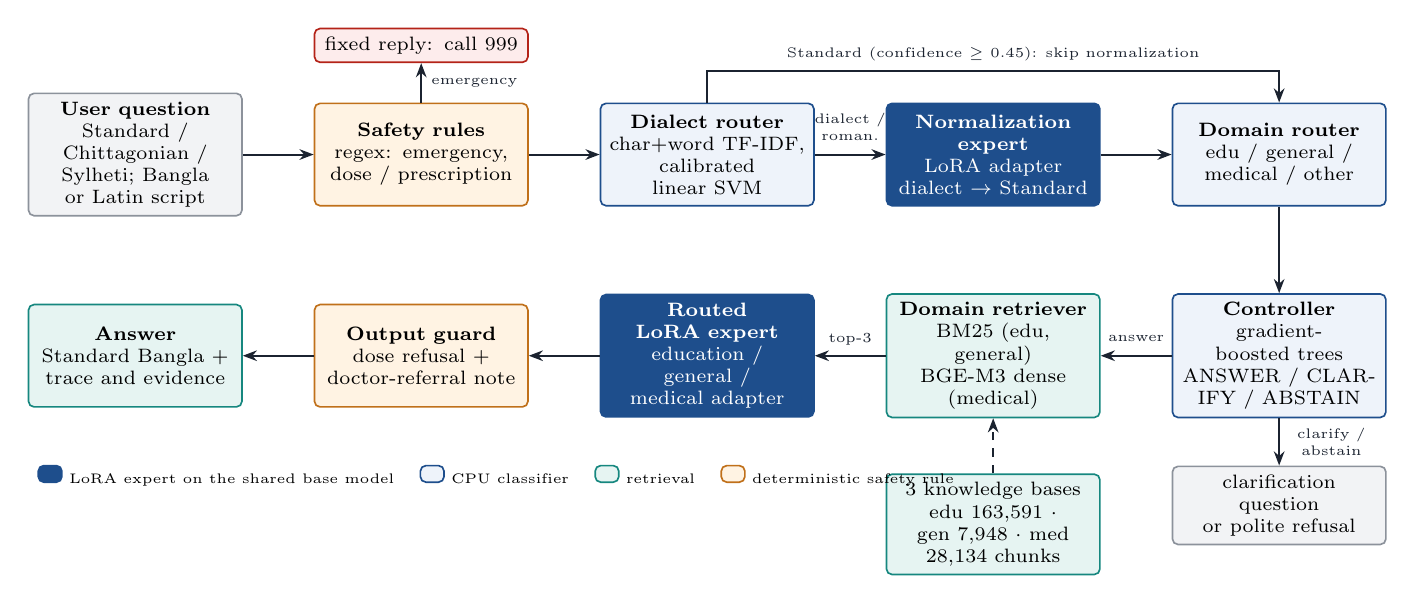
\begin{tikzpicture}[node distance=6mm and 9mm, every node/.style={font=\scriptsize}]
\tikzset{pbox/.style={box, minimum width=27mm, minimum height=13mm, text width=25mm}}
% row 1
\node[pbox, fill=greylt, draw=greyd] (q) {\textbf{User question}\\Standard / Chittagonian /\\Sylheti; Bangla or Latin script};
\node[pbox, safe, right=of q] (s) {\textbf{Safety rules}\\regex: emergency,\\dose / prescription};
\node[pbox, right=of s] (dr) {\textbf{Dialect router}\\char+word TF-IDF,\\calibrated linear SVM};
\node[pbox, lora, right=of dr] (n) {\textbf{Normalization expert}\\LoRA adapter\\dialect $\rightarrow$ Standard};
\node[pbox, right=of n] (dom) {\textbf{Domain router}\\edu / general /\\medical / other};
% row 2 (right to left)
\node[pbox, below=11mm of dom] (c) {\textbf{Controller}\\gradient-boosted trees\\ANSWER / CLARIFY / ABSTAIN};
\node[pbox, cpu, left=of c] (r) {\textbf{Domain retriever}\\BM25 (edu, general)\\BGE-M3 dense (medical)};
\node[pbox, lora, left=of r] (e) {\textbf{Routed LoRA expert}\\education / general /\\medical adapter};
\node[pbox, safe, left=of e] (g) {\textbf{Output guard}\\dose refusal +\\doctor-referral note};
\node[pbox, fill=teallt, draw=teal, left=of g] (a) {\textbf{Answer}\\Standard Bangla +\\trace and evidence};
% side nodes
\node[box, fill=redlt, draw=redd, above=5mm of s, text width=25mm] (em) {fixed reply: call 999};
\node[grey, below=6mm of c, text width=25mm] (cl) {clarification question\\or polite refusal};
% KBs
\node[cpu, below=7mm of r, text width=25mm, minimum height=9mm] (kb) {3 knowledge bases\\edu 163,591 $\cdot$ gen 7,948 $\cdot$ med 28,134 chunks};
% arrows
\draw[arr] (q) -- (s);
\draw[arr] (s) -- (dr);
\draw[arr] (dr) -- node[lab, above=0.5mm]{dialect /\\roman.} (n);
\draw[arr] (n) -- (dom);
\draw[arr] (dr.north) -- ++(0,4mm) -| node[lab, pos=0.25, above]{Standard (confidence $\ge$ 0.45): skip normalization} (dom.north);
\draw[arr] (s) -- node[lab, right]{emergency} (em);
\draw[arr] (dom) -- (c);
\draw[arr] (c) -- node[lab, above=0.5mm]{answer} (r);
\draw[arr] (r) -- node[lab, above]{top-3} (e);
\draw[arr] (e) -- (g);
\draw[arr] (g) -- (a);
\draw[arr] (c) -- node[lab, right=1mm]{clarify /\\abstain} (cl);
\draw[darr] (kb) -- (r);
% legend
\node[anchor=north west, font=\tiny] at ($(a.south west)+(0,-6mm)$) {\tikz\node[lora, minimum width=3mm, minimum height=2mm]{};~LoRA expert on the shared base model \quad
\tikz\node[box, minimum width=3mm, minimum height=2mm]{};~CPU classifier \quad
\tikz\node[cpu, minimum width=3mm, minimum height=2mm]{};~retrieval \quad
\tikz\node[safe, minimum width=3mm, minimum height=2mm]{};~deterministic safety rule};
\end{tikzpicture}
\caption{Inference pipeline. A question passes the safety rules, is routed by language variety, normalized if it is dialectal or romanized, routed by domain, checked by the controller, grounded in three passages from its domain's knowledge base, answered by that domain's LoRA expert and finally checked by the output guard. The two dark boxes are LoRA adapters on one shared 4-bit Gemma-4-E4B-it model and are the only steps that run the language model; everything else runs on a CPU.}
\label{fig:pipeline}
\end{figure}

\begin{table}[!t]
\centering
\caption{Research questions and the experiments (stages) that answer them.}
\label{tab:rq}
\scriptsize
\begin{tabularx}{\linewidth}{@{}l Y L{2.7cm}@{}}
\toprule
& Research question & Experiment (stage) \\
\midrule
RQ1 & How accurately, and with how well-calibrated confidence, can a lightweight router identify the variety and the domain? & router comparison incl.\ BanglaBERT (S4); routing inside the system (S5); human-written questions (S6) \\
RQ2 & How well can a fine-tuned model normalize dialect and romanized questions, and how much of the dialect gap does it close? & normalization benchmark, prompting baselines (S3, S5); \condt{FULL} vs \condt{NO\_NORMALIZATION} (S5); S6; S8 \\
RQ3 & What do retrieval, fine-tuned experts, domain routing and the controller contribute; do routed experts beat one shared adapter? & ablations \condt{NO\_RAG}, \condt{BASE\_MODEL}, \condt{NO\_DOMAIN\_ROUTING}, \condt{NO\_CONTROLLER}, \condt{POOLED\_ADAPTER} (S5) \\
RQ4 & Which open base model gives the best quality--cost balance, and does Bangla pre-training help after fine-tuning? & 7 models, identical QLoRA budget, 3 seeds for finalists (S2) \\
\bottomrule
\end{tabularx}
\end{table}

% =============================================================================
\section{Background}
\label{sec:background}

\subsection{Bangla Varieties and Dialect Normalization}
Standard Bangla (\tl{cholito bhasha}) is the variety of textbooks, news and administration. Regional varieties differ from it in pronunciation, vocabulary, verb endings and sometimes word order; Chittagonian (south-east) and Sylheti (north-east) are among the most divergent \cite{faria2023vashantor,jawad2026fivedialects}. Because there is no agreed dialect spelling, writers spell words as they are pronounced, and many type Bangla in Latin letters. \emph{Dialect normalization} rewrites a dialect sentence into Standard Bangla with the same meaning, so it is a form of machine translation \cite{faria2023vashantor}. Table~\ref{tab:words} shows word pairs from the training split of our dialect glossary: most everyday words change, which is why a system trained on Standard Bangla misreads dialect input.

\begin{table}[!t]
\centering
\caption{Dialect words and their Standard Bangla forms (transliterated; from the TRAIN split of the word-level glossary, Section~\ref{sec:v2}).}
\label{tab:words}
\scriptsize
\begin{tabular}{@{}llll@{}}
\toprule
Variety & Dialect form & Standard form & Meaning \\
\midrule
Chittagonian & \tl{\~ai} & \tl{ami} & I \\
Chittagonian & \tl{tun} & \tl{theke} & from \\
Chittagonian & \tl{baiddhe} & \tl{bedheche} & has tied \\
Sylheti & \tl{kita} & \tl{ki} & what \\
Sylheti & \tl{koilam} & \tl{bollam} & (I) said \\
Sylheti & \tl{jaimu} & \tl{jabo} & (I) will go \\
Sylheti & \tl{pushkuni} & \tl{pukur} & pond \\
\bottomrule
\end{tabular}
\end{table}

\subsection{Large Language Models and Instruction Tuning}
Modern language models are decoder-only Transformers \cite{vaswani2017attention} pre-trained to predict the next token and then instruction-tuned, i.e.\ fine-tuned on (instruction, response) pairs so that they follow a task description \cite{wei2022flan}. We phrase every task as a chat instruction in Bangla: a system message states the task, the user message carries the input, and the target is the desired output. A model's \emph{tokenizer fertility} (tokens per word) decides how long a Bangla sentence becomes and therefore the training cost and the context that fits.

\subsection{Low-Rank Adaptation (LoRA)}
Updating every weight of a billion-parameter model is expensive. LoRA \cite{hu2022lora} freezes a pretrained weight matrix $W_0\in\mathbb{R}^{d\times k}$ and learns a low-rank update:
\begin{equation}
h = W_0x + \Delta W x = W_0x + \frac{\alpha}{r}\,BAx,
\label{eq:lora}
\end{equation}
with $B\in\mathbb{R}^{d\times r}$, $A\in\mathbb{R}^{r\times k}$ and $r\ll\min(d,k)$.
Only $A$ and $B$ are trained ($r(d+k)$ instead of $dk$ values per matrix; $B$ starts at zero so training starts from the original model). Many adapters can be attached to one frozen base and switched per request (Fig.~\ref{fig:lora}). Our adapters use $r=16$, $\alpha=32$ in every attention and MLP projection: 34.9\,M trainable parameters (133\,MB) each.

\begin{figure}[!t]
\centering
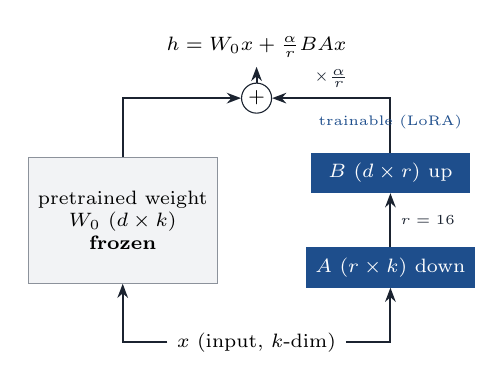
\begin{tikzpicture}[font=\scriptsize]
\node (x) at (0,0) {$x$ (input, $k$-dim)};
\node[draw=greyd, fill=greylt, minimum width=24mm, minimum height=16mm, align=center] (W) at (-1.7,1.55) {pretrained weight\\$W_0$ ($d\times k$)\\\textbf{frozen}};
\node[draw=navy, fill=navy, text=white, minimum width=20mm, minimum height=5mm] (A) at (1.7,0.95) {$A$ ($r\times k$) down};
\node[draw=navy, fill=navy, text=white, minimum width=20mm, minimum height=5mm] (B) at (1.7,2.15) {$B$ ($d\times r$) up};
\node[circle, draw=ink, inner sep=1pt] (plus) at (0,3.1) {$+$};
\node (h) at (0,3.75) {$h=W_0x+\frac{\alpha}{r}BAx$};
\draw[arr] (x) -| (W.south);
\draw[arr] (x) -| (A.south);
\draw[arr] (A) -- node[lab, right]{$r=16$} (B);
\draw[arr] (W.north) |- (plus.west);
\draw[arr] (B.north) |- node[lab, pos=0.75, above]{$\times\frac{\alpha}{r}$} (plus.east);
\draw[arr] (plus) -- (h);
\node[lab, text=navy, align=center] at (1.7,2.8) {trainable (LoRA)};
\end{tikzpicture}
\caption{LoRA: the pretrained weight stays frozen; only the low-rank matrices $A$ and $B$ are trained. Swapping $(A,B)$ swaps the skill while the base model stays in memory once.}
\label{fig:lora}
\end{figure}

\subsection{QLoRA: Fine-Tuning a Quantized Model}
QLoRA \cite{dettmers2023qlora} stores the frozen base in 4-bit NormalFloat (NF4), a data type whose 16 levels are quantiles of a normal distribution, so it fits normally distributed weights well; the quantization constants are themselves quantized (\emph{double quantization}). Gradients flow through the de-quantized weights into the LoRA matrices, which are kept in 16-bit precision. Fig.~\ref{fig:mem} shows the weight memory of a 4-billion-parameter model: NF4 needs about a quarter of the 16-bit memory, which is what lets one rented 48\,GB GPU train and serve every expert.

\begin{figure}[!t]
\centering
\resizebox{\linewidth}{!}{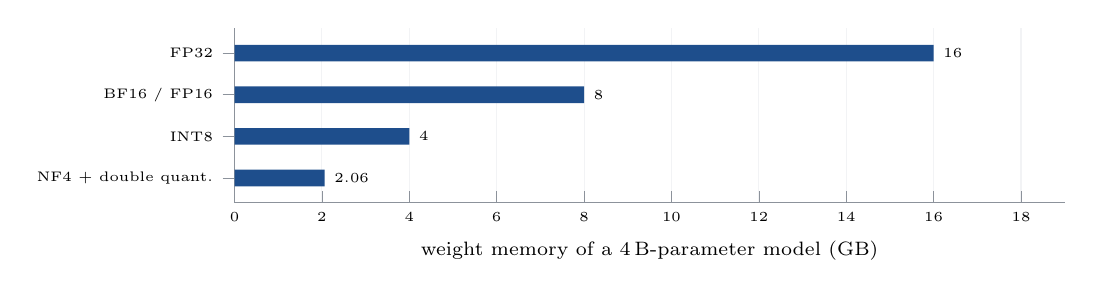
\begin{tikzpicture}
\begin{axis}[width=\linewidth, height=38mm, xbar, bar width=6pt, xmin=0, xmax=19,
  symbolic y coords={NF4 + double quant.,INT8,BF16 / FP16,FP32}, ytick=data, xlabel={weight memory of a 4\,B-parameter model (GB)},
  nodes near coords, nodes near coords style={font=\tiny, /pgf/number format/fixed, /pgf/number format/precision=2}, y dir=normal,
  enlarge y limits=0.2, xmajorgrids, ymajorgrids=false]
\addplot[fill=navy, draw=none] coordinates {(2.06,NF4 + double quant.) (4,INT8) (8,BF16 / FP16) (16,FP32)};
\end{axis}
\end{tikzpicture}}
\caption{Weight memory per numeric format for $4\times10^9$ parameters (bytes per parameter: FP32 4, BF16 2, INT8 1, NF4 with double quantization $\approx$4.127 bits \cite{dettmers2023qlora}). Activations, the LoRA weights and the optimizer come on top.}
\label{fig:mem}
\end{figure}

\subsection{Retrieval-Augmented Generation}
A language model that answers from memory can produce fluent but unsupported answers \cite{ji2023survey}. Retrieval-augmented generation (RAG) first retrieves passages relevant to the question and conditions the generator on them \cite{lewis2020rag} (Fig.~\ref{fig:rag}). Two kinds of retrievers are used.

\textbf{Sparse retrieval (BM25)} scores a document $d$ for a query $q$ by weighted term overlap \cite{robertson2009bm25}:
\begin{equation}
\mathrm{BM25}(q,d)=\sum_{t\in q}\mathrm{IDF}(t)\,\frac{f_{t,d}\,(k_1+1)}{f_{t,d}+k_1\big(1-b+b\,\frac{|d|}{\overline{|d|}}\big)},
\end{equation}
with $\mathrm{IDF}(t)=\ln\!\big(1+\frac{N-n_t+0.5}{n_t+0.5}\big)$, term frequency $f_{t,d}$, $N$ documents of which $n_t$ contain $t$, $k_1=1.2$ and $b=0.75$. We add light Bangla suffix stripping.

\textbf{Dense retrieval} encodes query and passage into vectors and ranks by cosine similarity $\cos(\mathbf{e}_q,\mathbf{e}_d)$ \cite{karpukhin2020dpr}; BGE-M3 \cite{chen2024bgem3} and multilingual-E5 \cite{wang2024me5} support Bangla. \textbf{Hybrid} retrieval fuses ranked lists with reciprocal rank fusion \cite{cormack2009rrf}:
\begin{equation}
\mathrm{RRF}(d)=\sum_{m}\frac{1}{k+\mathrm{rank}_m(d)},\qquad k=60.
\label{eq:rrf}
\end{equation}

\begin{figure}[!t]
\centering
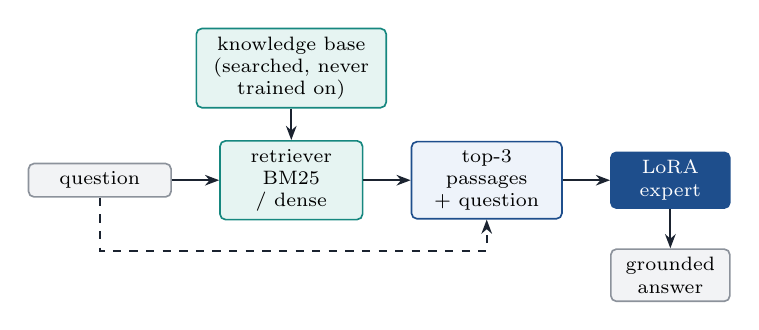
\begin{tikzpicture}[font=\scriptsize, node distance=5mm and 6mm]
\node[grey, text width=16mm] (q) {question};
\node[cpu, right=of q, text width=16mm] (ret) {retriever\\BM25 / dense};
\node[cpu, above=4mm of ret, text width=22mm] (kb) {knowledge base\\(searched, never trained on)};
\node[box, right=of ret, text width=17mm] (ctx) {top-3 passages\\+ question};
\node[lora, right=of ctx, text width=13mm] (gen) {LoRA\\expert};
\node[grey, below=5mm of gen, text width=13mm] (ans) {grounded\\answer};
\draw[arr] (q) -- (ret); \draw[arr] (kb) -- (ret); \draw[arr] (ret) -- (ctx); \draw[arr] (ctx) -- (gen); \draw[arr] (gen) -- (ans);
\draw[darr] (q.south) |- ([yshift=-4mm]ctx.south) -- (ctx.south);
\end{tikzpicture}
\caption{Retrieval-augmented generation: the expert answers from retrieved evidence, or writes a fixed ``not found'' sentence when the evidence does not contain the answer.}
\label{fig:rag}
\end{figure}

\subsection{Mixture of Experts and the Mixture-of-Adapters}
A mixture of experts combines specialised models through a gating function \cite{jacobs1991adaptive}; in modern LLMs, sparse MoE layers route each \emph{token} to a few expert sub-networks inside one model \cite{shazeer2017moe,fedus2022switch}. We apply the idea at the \emph{system} level (Fig.~\ref{fig:moa}): CPU routers send each \emph{question} to exactly one LoRA adapter on a shared base model (hard top-1 routing), closer to adapter-based transfer \cite{houlsby2019adapters} and to routed retrieval \cite{jeong2024adaptiverag,lee2025routerretriever} than to an MoE layer. The experts stay small, interpretable and replaceable.

\begin{figure}[!t]
\centering
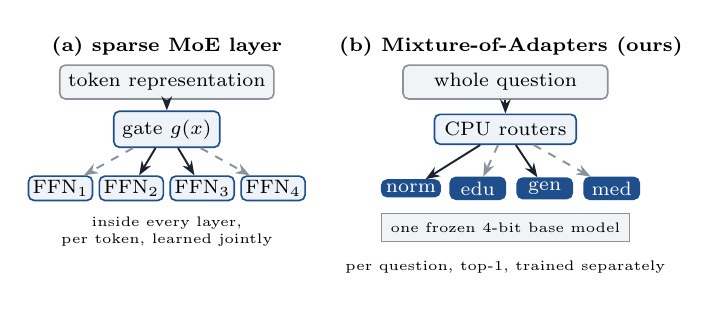
\begin{tikzpicture}[font=\tiny, node distance=2mm]
% left: token-level MoE
\node[font=\scriptsize\bfseries] at (0,2.35) {(a) sparse MoE layer};
\node[grey, minimum width=26mm] (tok) at (0,1.9) {token representation};
\node[box, minimum width=12mm] (gate) at (0,1.3) {gate $g(x)$};
\foreach \i/\xx in {1/-1.35,2/-0.45,3/0.45,4/1.35} { \node[box, minimum width=7mm, inner sep=1.5pt] (f\i) at (\xx,0.55) {FFN$_\i$}; }
\draw[arr] (tok) -- (gate);
\draw[arr] (gate) -- (f2); \draw[arr] (gate) -- (f3);
\draw[darr, draw=greyd] (gate) -- (f1); \draw[darr, draw=greyd] (gate) -- (f4);
\node[align=center] at (0,0.0) {inside every layer,\\per token, learned jointly};
% right: MoA
\node[font=\scriptsize\bfseries] at (4.37,2.35) {(b) Mixture-of-Adapters (ours)};
\node[grey, minimum width=26mm] (qq) at (4.3,1.9) {whole question};
\node[box, minimum width=18mm] (rt) at (4.3,1.3) {CPU routers};
\node[lora, minimum width=7mm, inner sep=1.5pt] (a1) at (3.1,0.55) {norm};
\node[lora, minimum width=7mm, inner sep=1.5pt] (a2) at (3.95,0.55) {edu};
\node[lora, minimum width=7mm, inner sep=1.5pt] (a3) at (4.8,0.55) {gen};
\node[lora, minimum width=7mm, inner sep=1.5pt] (a4) at (5.65,0.55) {med};
\draw[arr] (qq) -- (rt); \draw[arr] (rt) -- (a1); \draw[arr] (rt) -- (a3);
\draw[darr, draw=greyd] (rt) -- (a2); \draw[darr, draw=greyd] (rt) -- (a4);
\node[draw=greyd, fill=greylt, minimum width=27mm, minimum height=3mm] at (4.3,0.05) {one frozen 4-bit base model};
\node[align=center] at (4.3,-0.45) {per question, top-1, trained separately};
\end{tikzpicture}
\caption{Token-level sparse MoE vs.\ the system-level Mixture-of-Adapters used here: one adapter for rewriting, then the adapter of the predicted domain for answering.}
\label{fig:moa}
\end{figure}

\subsection{Calibrated Classifiers}
The routers must say \emph{how sure} they are, because low confidence changes what the system does. A linear support vector machine \cite{cortes1995svm} outputs a score $f(x)$, which sigmoid (Platt) calibration \cite{platt1999probabilistic} turns into a probability $P(y{=}1\mid x)=1/(1+\exp(Af(x)+B))$, with $A,B$ fitted on held-out folds. Calibration quality is measured by the expected calibration error \cite{guo2017calibration}:
\begin{equation}
\mathrm{ECE}=\sum_{m=1}^{M}\frac{|B_m|}{n}\,\big|\mathrm{acc}(B_m)-\mathrm{conf}(B_m)\big|,
\end{equation}
where the predictions are grouped into $M$ confidence bins $B_m$; a well-calibrated router is right 90\% of the time when it says 0.9.

\subsection{Selective Answering}
A realistic system must also recognise questions it should not answer. SQuAD~2.0 showed that models trained only on answerable questions answer unanswerable ones confidently \cite{rajpurkar2018squad2}, and selective QA trades coverage for accuracy by abstaining when unsure \cite{kamath2020selective}. Our design separates three cases: the question is out of scope or vague (the controller asks or refuses), the evidence lacks the answer (the expert writes a fixed ``not found'' sentence, learned from real unanswerable questions), or it is an emergency (a fixed safety reply).

% =============================================================================
\section{Overall Workflow}
\label{sec:overview}

The methodology follows \emph{compare $\rightarrow$ adapt $\rightarrow$ route $\rightarrow$ evaluate}. We compare open base models under an identical fine-tuning budget, adapt the winner into LoRA experts, build the routers, retrievers, controller and safety layer around them, and evaluate the whole system and its ablations on the same questions in three varieties. The work runs as staged notebooks (Fig.~\ref{fig:workflow}): stages that only need a CPU run on free Colab runtimes, and stages that train or run the language model run as resumable background jobs on one rented NVIDIA A40 (48\,GB). Stage outputs move between the two through a private Hugging Face dataset repository with SHA-256 manifests. Algorithm~\ref{alg:infer} summarises inference.

\begin{figure}[!t]
\centering
\resizebox{\linewidth}{!}{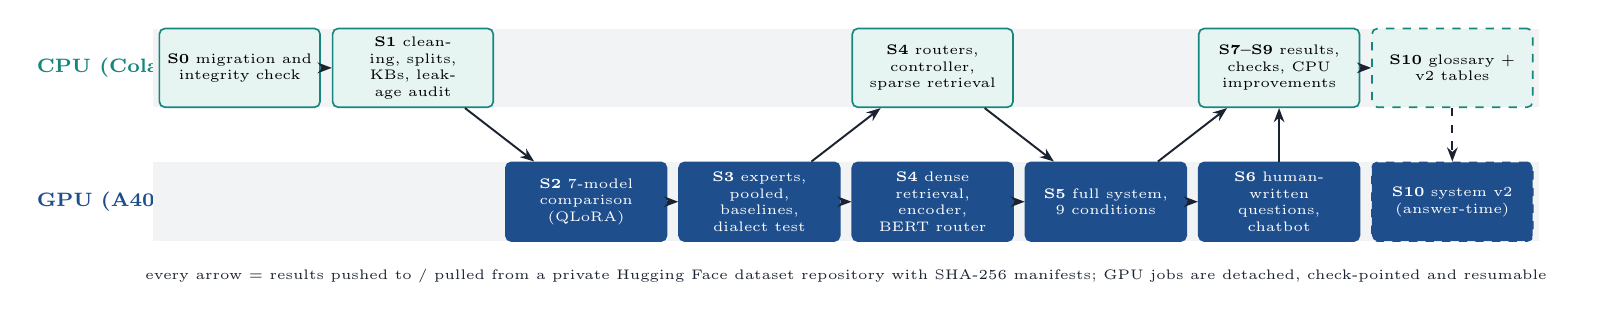
\begin{tikzpicture}[font=\tiny]
\tikzset{st/.style={draw, rounded corners=2pt, align=center, minimum height=10mm, text width=19mm, inner sep=2pt, line width=0.6pt}}
\node[font=\scriptsize\bfseries, text=teal, anchor=west] at (-1.9,1.2) {CPU (Colab)};
\node[font=\scriptsize\bfseries, text=navy, anchor=west] at (-1.9,-0.5) {GPU (A40)};
\draw[draw=greylt, line width=10mm] (-0.3,1.2) -- (17.3,1.2);
\draw[draw=greylt, line width=10mm] (-0.3,-0.5) -- (17.3,-0.5);
\node[st, fill=teallt, draw=teal] (s0) at (0.8,1.2) {\textbf{S0} migration and\\integrity check};
\node[st, fill=teallt, draw=teal] (s1) at (3.0,1.2) {\textbf{S1} cleaning, splits,\\KBs, leakage audit};
\node[st, fill=navy, text=white, draw=navy] (s2) at (5.2,-0.5) {\textbf{S2} 7-model\\comparison (QLoRA)};
\node[st, fill=navy, text=white, draw=navy] (s3) at (7.4,-0.5) {\textbf{S3} experts, pooled,\\baselines, dialect test};
\node[st, fill=teallt, draw=teal] (s4a) at (9.6,1.2) {\textbf{S4} routers, controller,\\sparse retrieval};
\node[st, fill=navy, text=white, draw=navy] (s4b) at (9.6,-0.5) {\textbf{S4} dense retrieval,\\encoder, BERT router};
\node[st, fill=navy, text=white, draw=navy] (s5) at (11.8,-0.5) {\textbf{S5} full system,\\9 conditions};
\node[st, fill=navy, text=white, draw=navy] (s6) at (14.0,-0.5) {\textbf{S6} human-written\\questions, chatbot};
\node[st, fill=teallt, draw=teal] (s78) at (14.0,1.2) {\textbf{S7--S9} results,\\checks, CPU improvements};
\node[st, fill=navy, text=white, draw=navy, dashed] (s10) at (16.2,-0.5) {\textbf{S10} system v2\\(answer-time)};
\node[st, fill=teallt, draw=teal, dashed] (s10c) at (16.2,1.2) {\textbf{S10} glossary +\\v2 tables};
\draw[arr] (s0) -- (s1); \draw[arr] (s1) -- (s2); \draw[arr] (s2) -- (s3); \draw[arr] (s3) -- (s4a);
\draw[arr] (s3) -- (s4b); \draw[arr] (s4a) -- (s5); \draw[arr] (s4b) -- (s5); \draw[arr] (s5) -- (s6);
\draw[arr] (s6) -- (s78); \draw[arr] (s5) -- (s78); \draw[darr] (s78) -- (s10c); \draw[darr] (s10c) -- (s10);
\node[align=center, font=\tiny, text=ink] at (8.5,-1.45) {every arrow = results pushed to / pulled from a private Hugging Face dataset repository with SHA-256 manifests; GPU jobs are detached, check-pointed and resumable};
\end{tikzpicture}}
\caption{Development workflow. Teal stages run on a CPU, dark stages on one rented A40 GPU; dashed stages are the optional DEV-selected improvements (Section~\ref{sec:v2}). About 40 GPU-hours (US\$20) were used up to S6.}
\label{fig:workflow}
\end{figure}

\begin{algorithm}[!t]
\caption{Answering one question}
\label{alg:infer}
\footnotesize
\begin{algorithmic}[1]
\Require question $q$; routers $R_{\mathrm{var}},R_{\mathrm{dom}}$; controller $C$; KBs $\mathcal{K}_d$; experts $E_{\mathrm{norm}},E_d$
\If{$\mathrm{Emergency}(q)$} \Return fixed emergency reply (call 999) \EndIf
\State $(v,p_v)\gets R_{\mathrm{var}}(q)$ \Comment{Standard / Chittagonian / Sylheti}
\If{($v\neq$ Standard \textbf{and} $p_v\ge 0.45$) \textbf{or} $q$ is romanized}
  \State $\hat q\gets E_{\mathrm{norm}}(q, v)$ \Comment{LoRA normalization}
\Else \State $\hat q\gets q$ \EndIf
\If{$\mathrm{Emergency}(\hat q)$} \Return fixed emergency reply \EndIf
\State $(d,p_d)\gets R_{\mathrm{dom}}(\hat q)$ \Comment{edu / general / medical / other}
\State $a\gets C(\text{router probabilities, BM25 signals, text features})$
\If{$a=$ CLARIFY} \Return clarification question \EndIf
\If{$a=$ ABSTAIN \textbf{or} $d=$ other} \Return polite refusal \EndIf
\State $P\gets$ top-3 passages of $\hat q$ in $\mathcal{K}_d$ \Comment{BM25 or dense}
\State $y\gets E_d(P,\hat q)$ \Comment{expert of domain $d$; may say ``not found''}
\If{$d=$ medical} \State $y\gets$ [dose refusal if requested] $+\,y\,+$ doctor-referral note \EndIf
\State \Return $y$ with trace $(v,p_v,\hat q,d,a,P)$
\end{algorithmic}
\end{algorithm}

% =============================================================================
\section{Data}
\label{sec:data}

\subsection{Three Data Roles}
Fig.~\ref{fig:roles} shows how the data are separated. \emph{Training data} change model weights: dialect--Standard pairs, the training splits of the QA datasets, and the router and controller data. \emph{Knowledge} is only searched at answer time: textbook chunks, Wikipedia passages, doctor answers from the training split, and drug and disease descriptions. \emph{Evaluation data} are held out: DEV for every choice, TEST once for reporting.

\begin{figure}[!t]
\centering
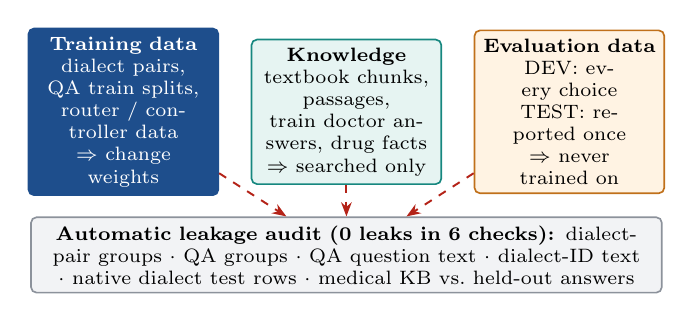
\begin{tikzpicture}[font=\tiny, node distance=3mm]
\node[lora, text width=22mm, minimum height=15mm] (tr) {\textbf{Training data}\\dialect pairs, QA train splits,\\router / controller data\\$\Rightarrow$ change weights};
\node[cpu, text width=22mm, minimum height=15mm, right=4mm of tr] (kn) {\textbf{Knowledge}\\textbook chunks, passages,\\train doctor answers, drug facts\\$\Rightarrow$ searched only};
\node[safe, text width=22mm, minimum height=15mm, right=4mm of kn] (ev) {\textbf{Evaluation data}\\DEV: every choice\\TEST: reported once\\$\Rightarrow$ never trained on};
\node[grey, text width=78mm, below=4mm of kn] (au) {\textbf{Automatic leakage audit (0 leaks in 6 checks):} dialect-pair groups $\cdot$ QA groups $\cdot$ QA question text $\cdot$ dialect-ID text $\cdot$ native dialect test rows $\cdot$ medical KB vs.\ held-out answers};
\draw[darr, draw=redd] (tr) -- (au); \draw[darr, draw=redd] (kn) -- (au); \draw[darr, draw=redd] (ev) -- (au);
\end{tikzpicture}
\caption{The three data roles and the audit that keeps them apart. Test passages of NCTB-QA and BanglaRQA are in the KB (open-book QA needs them), but test questions and medical test answers never are.}
\label{fig:roles}
\end{figure}

\subsection{Sources}
Table~\ref{tab:datasets} lists every source and its role. Dialect data come from Vashantor \cite{faria2023vashantor}, Kothon \cite{kothon2026} and the ChatgaiyyaBench corpus \cite{chatgaiyyabench2026}, which contains the ChatgaiyyaAlap \cite{chatgaiyyaalap2025}, ONUBAD \cite{sultana2025onubad} and BD-dialect sentences. The Mendeley release of ChatgaiyyaAlap (\texttt{Dataset\_Chittagong\_2.0.csv}) holds the same sentences as the ChatgaiyyaAlap part of ChatgaiyyaBench, so all of its rows were removed as duplicates. Fig.~\ref{fig:sources} shows how many dialect--Standard pairs each source contributes after cleaning.

\begin{table}[!t]
\centering
\caption{Data sources, rows used, and role (``rows used'' are counted before cross-source de-duplication; Fig.~\ref{fig:sources} shows the unique pairs).}
\label{tab:datasets}
\scriptsize
\begin{tabularx}{\textwidth}{@{}L{7.2cm} r Y@{}}
\toprule
Source & Rows used & Role \\
\midrule
Vashantor \cite{faria2023vashantor} (Chittagong, Sylhet; Barishal, Mymensingh, Noakhali) & 12,498 & dialect pairs incl.\ romanized; the three other regions are held out as \emph{unseen} dialects (test only) \\
Kothon \cite{kothon2026} (Chittagonian, Sylheti) & 17,328 & dialect pairs (native annotated) \\
ChatgaiyyaBench corpus \cite{chatgaiyyabench2026} (ChatgaiyyaAlap \cite{chatgaiyyaalap2025}, ONUBAD \cite{sultana2025onubad}, BD-dialect sentences; translation benchmark; romanized) & 21,614 & Chittagonian and Sylheti pairs, romanized pairs; its translation benchmark is test only \\
ChatgaiyyaAlap, Mendeley release (\texttt{Dataset\_Chittagong\_2.0.csv}) & 0 new & identical to the ChatgaiyyaAlap part of ChatgaiyyaBench: removed as duplicates \\
Local Language Dataset (regional dialects) & 1,007 & unverified pairs: \emph{training only}, never evaluated \\
NCTB-QA \cite{nctbqa} & 87,805 & education QA with unanswerable questions (official split) + KB passages \\
BanglaRQA \cite{ekram2022banglarqa} & 14,889 & general-knowledge QA (official split) + KB passages \\
Bangla national-curriculum textbooks & 131,361 & education KB chunks (retrieval only) \\
Doctor QA (Bangla) & 4,417 & medical QA (80/10/10 grouped split) + KB (training answers only) \\
Bangla-MedER \cite{aurpa2026banglameder}; Medicine dataset of Bangladesh; healthcare-chatbot intents & 24,725 & medical KB (retrieval only) \\
Bangla-HealthNER \cite{khan2023nervous}; specialist classification; BanglaCHQ-Summ questions \cite{khan2023banglachqsumm} & 25,782 & domain-router data \\
Out-of-scope news and blog sentences & 8,006 & domain router ``other'' class \\
BEnQA \cite{shafayat2024benqa}; Bangla-MMLU sample; BanglaMedQA \cite{banglamedqa} & 8,075 & multiple-choice probes (evaluation only) \\
ChatgaiyyaBench QA cloze & 590 & native Chittagonian comprehension probe (evaluation only) \\
\bottomrule
\end{tabularx}
\end{table}

\begin{figure}[!t]
\centering
\resizebox{\linewidth}{!}{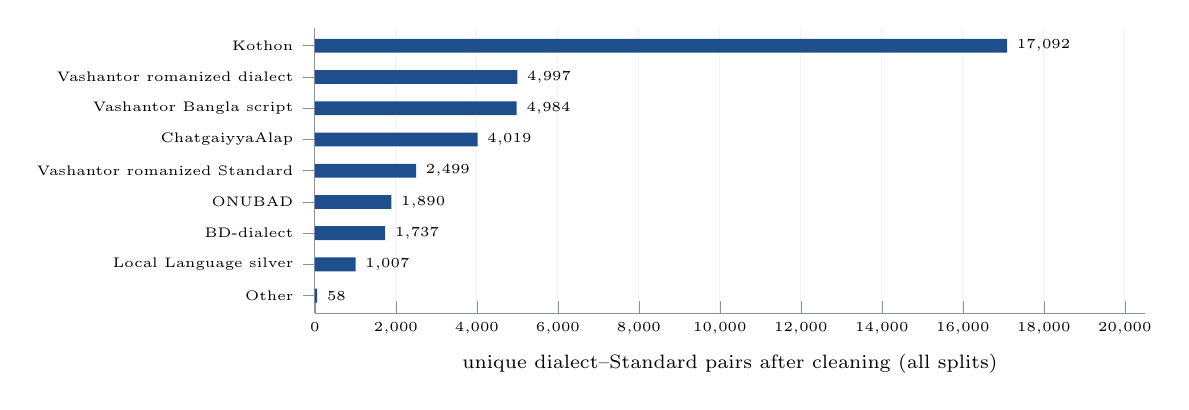
\begin{tikzpicture}
\begin{axis}[width=\linewidth, height=52mm, xbar, bar width=5pt, xmin=0, xmax=20500,
  symbolic y coords={Other,Local Language silver,BD-dialect,ONUBAD,Vashantor romanized Standard,ChatgaiyyaAlap,Vashantor Bangla script,Vashantor romanized dialect,Kothon},
  ytick=data, xlabel={unique dialect--Standard pairs after cleaning (all splits)},
  nodes near coords, nodes near coords style={font=\tiny}, enlarge y limits=0.07, xmajorgrids, ymajorgrids=false,
  scaled x ticks=false, xticklabel style={/pgf/number format/fixed}]
\addplot[fill=navy, draw=none] coordinates {(58,Other) (1007,Local Language silver) (1737,BD-dialect) (1890,ONUBAD) (2499,Vashantor romanized Standard) (4019,ChatgaiyyaAlap) (4984,Vashantor Bangla script) (4997,Vashantor romanized dialect) (17092,Kothon)};
\end{axis}
\end{tikzpicture}}
\caption{Unique dialect--Standard pairs per source after cleaning and cross-source de-duplication (38,283 in total; 16,905 Chittagonian and 13,855 Sylheti in Bangla script, 7,523 romanized).}
\label{fig:sources}
\end{figure}

\subsection{Exploratory Data Analysis}
The dialects differ strongly from Standard Bangla at the surface (Fig.~\ref{fig:divergence} and Fig.~\ref{fig:overlap}). A Chittagonian sentence keeps only 29.6\% of the words and 43.0\% of the character trigrams of its Standard translation; for Sylheti the figures are 36.5\% and 49.4\%. Measured as Jaccard similarity (shared trigrams divided by \emph{all} distinct trigrams of both sentences), the overlap is 0.296 and 0.348, so Chittagonian is the harder variety. Sentences are short (about 6--7 words), so changing two or three words already removes half of the trigrams. Romanized questions share no words with Bangla-script text at all, because they use another alphabet, which is why romanized input is always normalized. The QA data differ by domain: education questions average 9.8 words with 10.4-word answers, general questions 8.2 and 5.2 words, and medical questions 18.6 words with 50.1-word doctor answers; 43\% of education and 24\% of general questions are unanswerable, which gives real training signal for abstention.

\begin{figure}[!t]
\centering
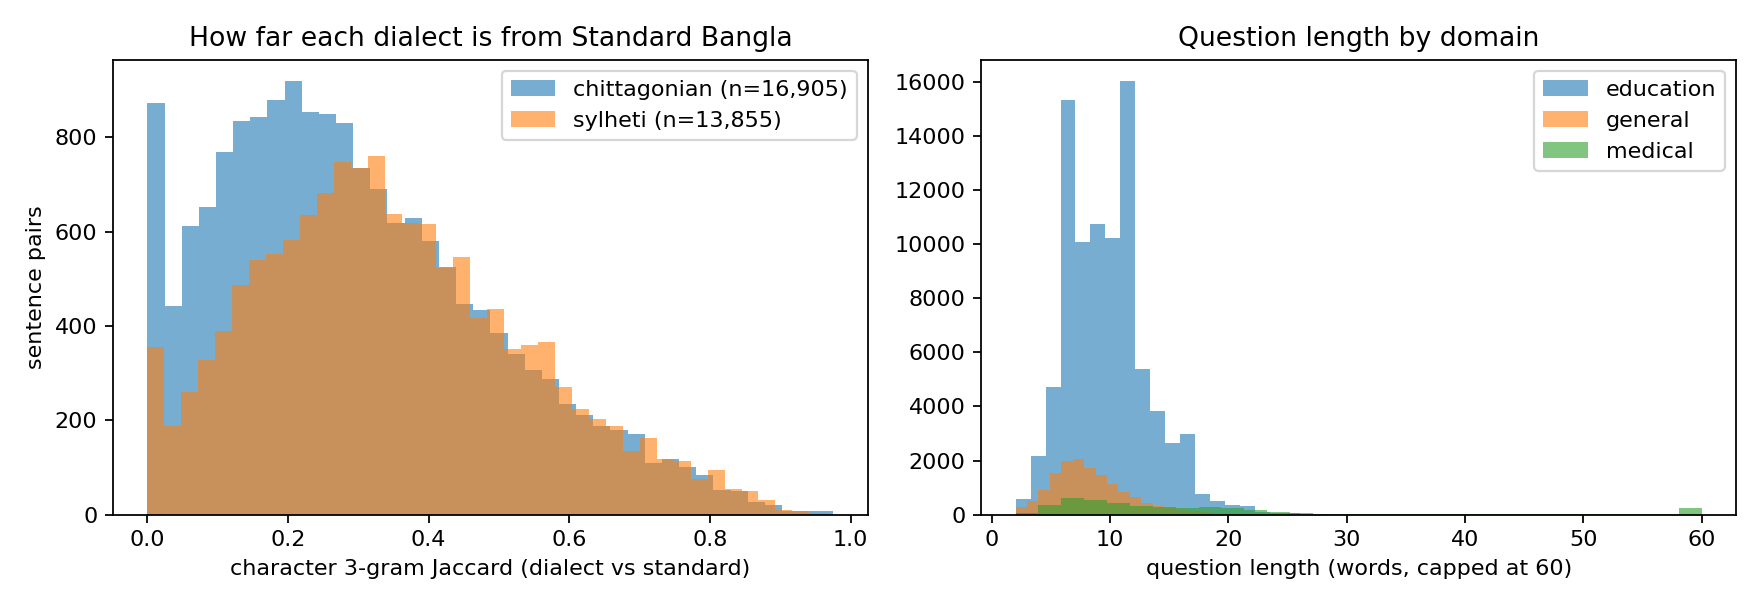
\includegraphics[width=0.66\textwidth]{fig_dialect_divergence.png}\hfill
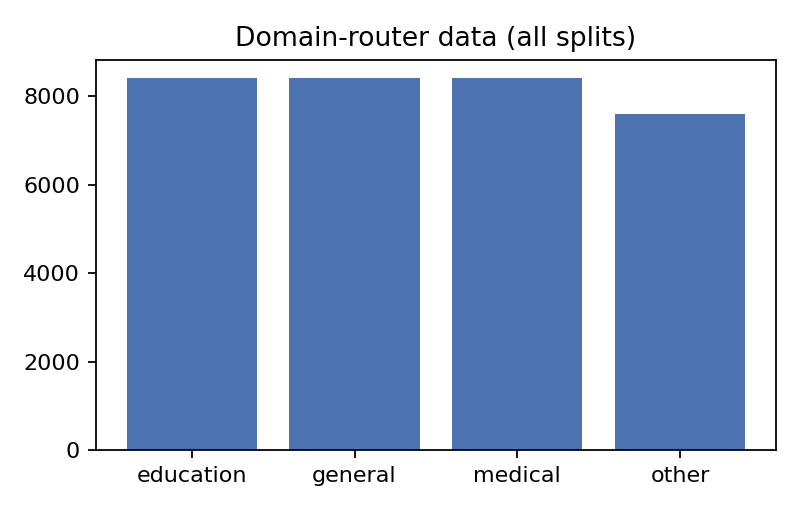
\includegraphics[width=0.30\textwidth]{fig_domain_distribution.png}
\caption{Left: character 3-gram Jaccard between each dialect sentence and its Standard translation (a peak near 0 means almost every trigram changed), and question length per domain. Right: the balanced domain-router data.}
\label{fig:divergence}
\end{figure}

\begin{figure}[!t]
\centering
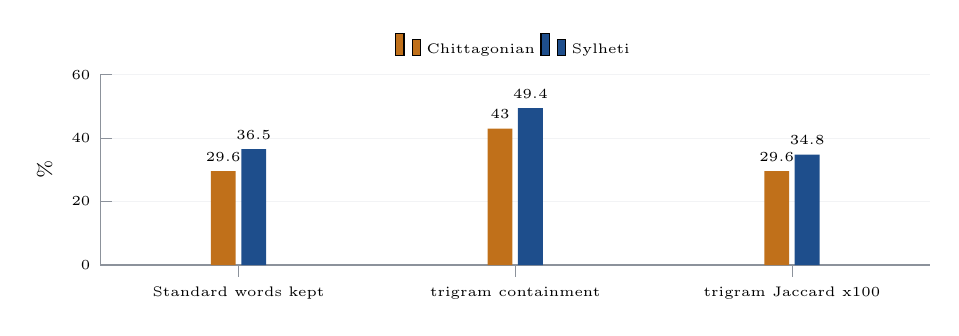
\begin{tikzpicture}
\begin{axis}[width=\linewidth, height=40mm, ybar, bar width=9pt, ymin=0, ymax=60,
  symbolic x coords={Standard words kept,trigram containment,trigram Jaccard x100}, xtick=data,
  ylabel={\%}, enlarge x limits=0.25, legend style={at={(0.5,1.03)}, anchor=south}, legend columns=2,
  nodes near coords, nodes near coords style={font=\tiny, /pgf/number format/fixed, /pgf/number format/precision=1}]
\addplot[fill=amber, draw=none] coordinates {(Standard words kept,29.6) (trigram containment,43.0) (trigram Jaccard x100,29.6)};
\addplot[fill=navy, draw=none] coordinates {(Standard words kept,36.5) (trigram containment,49.4) (trigram Jaccard x100,34.8)};
\legend{Chittagonian, Sylheti}
\end{axis}
\end{tikzpicture}
\caption{How much of the Standard sentence survives in the dialect sentence (Bangla-script pairs, all splits).}
\label{fig:overlap}
\end{figure}

\subsection{Cleaning}
All text is Unicode-NFC normalized; invisible characters (zero-width space, soft hyphen, byte-order mark) are removed while the joiners Bangla needs are kept. Fig.~\ref{fig:cleaning} lists the removals. Word-level dictionary entries are removed from the \emph{training} pairs because the normalization expert rewrites whole questions, and 10k one-word examples would teach context-free word swaps and very short outputs; they were reused later, differently, as a glossary of 2,356 Chittagonian and 974 Sylheti entries (TRAIN split only), which was tested in system v2 (Section~\ref{sec:v2}). Pairs whose dialect text equals the Standard text carry no dialect signal and would give the dialect router the same sentence with two labels.

\begin{figure}[!t]
\centering
\resizebox{\linewidth}{!}{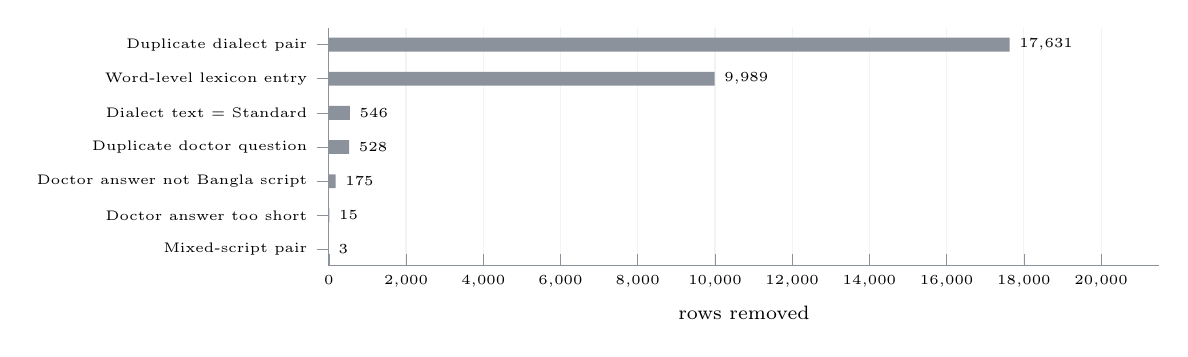
\begin{tikzpicture}
\begin{axis}[width=\linewidth, height=46mm, xbar, bar width=5pt, xmin=0, xmax=21500, xmode=normal,
  symbolic y coords={Mixed-script pair,Doctor answer too short,Doctor answer not Bangla script,Duplicate doctor question,Dialect text = Standard,Word-level lexicon entry,Duplicate dialect pair},
  ytick=data, xlabel={rows removed}, nodes near coords, nodes near coords style={font=\tiny},
  enlarge y limits=0.08, xmajorgrids, ymajorgrids=false, scaled x ticks=false]
\addplot[fill=greyd, draw=none] coordinates {(3,Mixed-script pair) (15,Doctor answer too short) (175,Doctor answer not Bangla script) (528,Duplicate doctor question) (546,Dialect text = Standard) (9989,Word-level lexicon entry) (17631,Duplicate dialect pair)};
\end{axis}
\end{tikzpicture}}
\caption{Cleaning log. Duplicates dominate: ChatgaiyyaBench re-distributes Vashantor and ChatgaiyyaAlap sentences. Doctor QA shrinks from 5,135 to 4,417 pairs.}
\label{fig:cleaning}
\end{figure}

\subsection{Transformation}
Every task becomes a chat instruction (system message, user message, target), written in Bangla so that the model answers in Bangla. Normalization prompts name the variety (``variety: Chittagonian; sentence: \ldots''); QA prompts contain three retrieved passages followed by the question. To teach grounded behaviour, the QA training targets follow the mix in Fig.~\ref{fig:mix}: 25\% of examples are real unanswerable questions and 8\% are \emph{retrieval misses} (the gold passage removed), both with a fixed ``the answer was not found in the given information'' target. Knowledge-base passages are split into overlapping windows of 110 words (stride 90) for NCTB-QA and BanglaRQA passages and 128 words for textbook rows (about 93--95 words on average); medical documents are stored as question--answer pairs or entity descriptions (about 27 words).

\begin{figure}[!t]
\centering
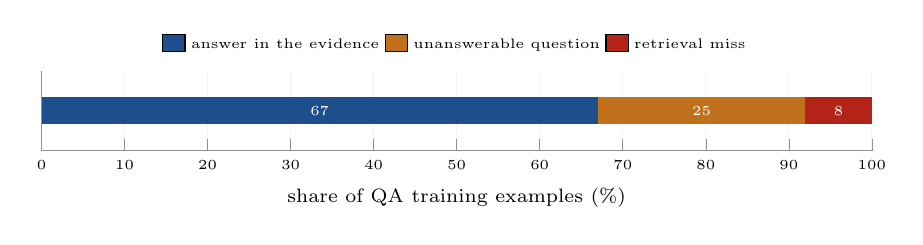
\begin{tikzpicture}
\begin{axis}[width=\linewidth, height=26mm, xbar stacked, bar width=10pt, xmin=0, xmax=100, ytick=\empty,
  xlabel={share of QA training examples (\%)}, legend style={at={(0.5,1.08)}, anchor=south, legend columns=3},
  ymajorgrids=false, xmajorgrids, nodes near coords, nodes near coords style={font=\tiny, text=white}]
\addplot[fill=navy, draw=none] coordinates {(67,0)};
\addplot[fill=amber, draw=none] coordinates {(25,0)};
\addplot[fill=redd, draw=none] coordinates {(8,0)};
\legend{answer in the evidence, unanswerable question, retrieval miss}
\end{axis}
\end{tikzpicture}
\caption{Target mix of the QA experts' training data: a third of the targets teach the expert to say ``not found'' instead of guessing (RAFT-style training \cite{zhang2024raft}).}
\label{fig:mix}
\end{figure}

\subsection{Integration, Splits and Reduction}
The dialect sources are merged into one pair table with provenance and split by \emph{group}: all versions of the same Standard sentence stay in one split (80/8/12), so no Standard sentence is seen in training and testing. Official splits (Vashantor, NCTB-QA, BanglaRQA, ChatgaiyyaBench benchmarks) are preserved, and a question text may never appear in two splits. Training sets are capped to fit the GPU budget: 24,000 normalization pairs, 11,943 education, 7,994 general and all 3,513 medical examples. Unverified silver data are used for training only. Table~\ref{tab:splits} gives the resulting splits and Table~\ref{tab:kb} the knowledge bases.

\begin{table}[!t]
\centering
\caption{Leak-free split sizes.}
\label{tab:splits}
\scriptsize
\begin{tabular}{@{}llrrr@{}}
\toprule
Task & Subset & Train & DEV & TEST \\
\midrule
\multirow{3}{*}{Dialect pairs} & Chittagonian & 16,030 & 1,411 & 1,968 \\
 & Sylheti & 13,119 & 1,295 & 1,961 \\
 & Standard (romanized) & 1,874 & 250 & 375 \\
\multirow{3}{*}{Dialect ID} & Chittagonian & 12,000 & 1,403 & 1,957 \\
 & Standard & 12,000 & 2,000 & 2,000 \\
 & Sylheti & 12,000 & 1,275 & 1,947 \\
Domain router & 4 classes & 6,000 each & 1,200 & 1,200 \\
\multirow{3}{*}{QA} & Education & 70,303 & 8,119 & 8,489 \\
 & General & 11,912 & 1,441 & 1,446 \\
 & Medical & 3,513 & 433 & 471 \\
MCQ (eval only) & 3 benchmarks & -- & 2,457 & 5,618 \\
Controller & 3 decisions & -- & 1,127 & 1,857 \\
\bottomrule
\end{tabular}
\end{table}

\begin{table}[!t]
\centering
\caption{Knowledge bases (searched, never trained on).}
\label{tab:kb}
\scriptsize
\resizebox{\linewidth}{!}{%
\begin{tabular}{@{}lrrr@{}}
\toprule
KB & Chunks & Documents & Avg.\ words \\
\midrule
Education (NCTB-QA passages + textbooks) & 163,591 & 96,907 & 93.2 \\
General (BanglaRQA passages) & 7,948 & 2,996 & 94.9 \\
Medical (doctor answers, MedER, drugs, intents) & 28,134 & 28,134 & 26.9 \\
Medical evaluation pool (retrieval benchmark only) & 904 & 904 & 48.7 \\
\bottomrule
\end{tabular}}
\end{table}

% =============================================================================
\section{Base-Model Selection}
\label{sec:models}

Seven open models were compared (Table~\ref{tab:candidates}): six instruction-tuned models and one Bangla base model. They include two \emph{Bangla-adapted vs.\ original} pairs (TigerLLM-1B \cite{raihan2025tigerllm} vs.\ Gemma-3-1B \cite{gemma3}; TituLM-3B \cite{titulm2025} vs.\ Llama-3.2-3B \cite{meta2024llama32}) to test whether Bangla continued pre-training still helps after task fine-tuning. The released TigerLLM-1B checkpoint has the architecture and tokenizer of Gemma-3-1B (identical fertility in Fig.~\ref{fig:fertility}), so Gemma-3-1B is its original model. Tokenizer fertility was measured first (Fig.~\ref{fig:fertility}): models that need 6--7 tokens per Bangla word make every example 4--5 times longer, which raises training time and forced a 4,096-token limit so that no long medical example is silently dropped.

\begin{table}[!t]
\centering
\caption{Candidate base models.}
\label{tab:candidates}
\scriptsize
\begin{tabular}{@{}lrc@{}}
\toprule
Model & Params (B) & Bangla-adapted \\
\midrule
TigerLLM-1B-it \cite{raihan2025tigerllm} & 1.0 & yes \\
Gemma-3-1B-it \cite{gemma3} & 1.0 & no \\
TituLM-Llama-3.2-3B \cite{titulm2025} & 3.2 & yes (base model) \\
Llama-3.2-3B-Instruct \cite{meta2024llama32} & 3.2 & no \\
Tiny-Aya-Fire \cite{tinyaya} & 3.35 & no \\
Qwen3-4B-Instruct-2507 \cite{qwen3} & 4.0 & no \\
Gemma-4-E4B-it \cite{gemma4} & 4.0 & no \\
\bottomrule
\end{tabular}
\end{table}

\begin{figure}[!t]
\centering
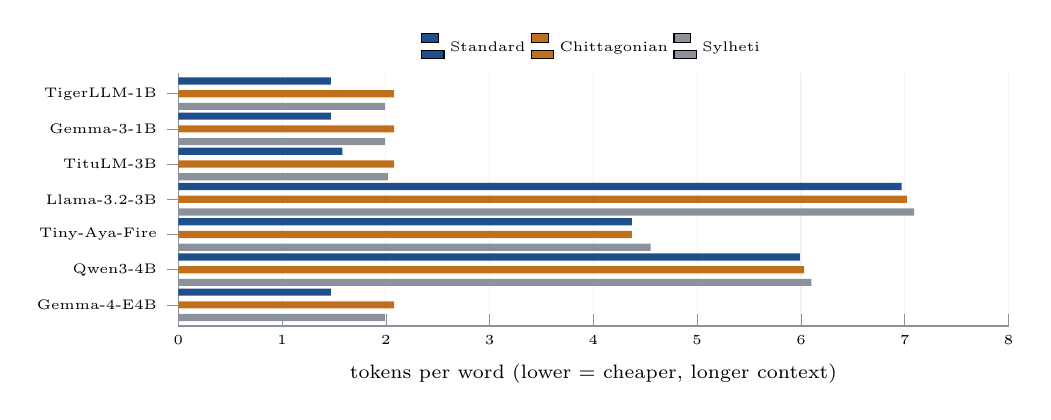
\begin{tikzpicture}
\begin{axis}[width=\linewidth, height=48mm, xbar, bar width=2.6pt, xmin=0, xmax=8,
  symbolic y coords={Gemma-4-E4B,Qwen3-4B,Tiny-Aya-Fire,Llama-3.2-3B,TituLM-3B,Gemma-3-1B,TigerLLM-1B},
  ytick=data, xlabel={tokens per word (lower = cheaper, longer context)}, enlarge y limits=0.1,
  legend style={at={(0.5,1.02)}, anchor=south}, legend columns=3, xmajorgrids, ymajorgrids=false, reverse legend]
\addplot[fill=greyd, draw=none] coordinates {(1.99,Gemma-4-E4B) (6.10,Qwen3-4B) (4.55,Tiny-Aya-Fire) (7.09,Llama-3.2-3B) (2.02,TituLM-3B) (1.99,Gemma-3-1B) (1.99,TigerLLM-1B)};
\addplot[fill=amber, draw=none] coordinates {(2.08,Gemma-4-E4B) (6.03,Qwen3-4B) (4.37,Tiny-Aya-Fire) (7.02,Llama-3.2-3B) (2.08,TituLM-3B) (2.08,Gemma-3-1B) (2.08,TigerLLM-1B)};
\addplot[fill=navy, draw=none] coordinates {(1.47,Gemma-4-E4B) (5.99,Qwen3-4B) (4.37,Tiny-Aya-Fire) (6.97,Llama-3.2-3B) (1.58,TituLM-3B) (1.47,Gemma-3-1B) (1.47,TigerLLM-1B)};
\legend{Sylheti, Chittagonian, Standard}
\end{axis}
\end{tikzpicture}
\caption{Tokenizer fertility on Standard, Chittagonian and Sylheti text. Dialect text costs 30--40\% more tokens than Standard text for the Gemma tokenizers.}
\label{fig:fertility}
\end{figure}

\textbf{Identical budget.} Every candidate receives the same QLoRA budget: 400 optimizer steps on the same 6,800 mixed-task examples, the same LoRA configuration, learning-rate schedule and seed. All candidates are evaluated zero-shot and after fine-tuning on a shared benchmark, and the choice uses a DEV composite
\begin{equation}
S=\tfrac{1}{5}\Big(\tfrac{\mathrm{chrF}_{\mathrm{ctg}}}{100}+\tfrac{\mathrm{chrF}_{\mathrm{syl}}}{100}+F1_{\mathrm{edu}}+F1_{\mathrm{gen}}+\tfrac{\mathrm{chrF}_{\mathrm{med}}}{100}\Big),
\end{equation}
where the first two terms are normalization quality and the rest are QA quality. The two finalists are re-trained with three seeds and compared with paired randomization tests; the winner (Gemma-4-E4B-it) hosts every expert.

% =============================================================================
\section{System Components}
\label{sec:components}

\subsection{Safety Layer}
Regular expressions written for Standard Bangla, Chittagonian, Sylheti and romanized Bangla detect emergencies (e.g.\ chest pain with breathlessness, unconsciousness, poisoning, stroke signs, suicidal statements) and dose or prescription requests. They run twice, on the raw and on the normalized question (Fig.~\ref{fig:safety}). Emergencies bypass the language model and return a fixed message asking the user to call the national emergency number 999 or go to the nearest hospital. No language model decides safety.

\begin{figure}[!t]
\centering
\resizebox{\linewidth}{!}{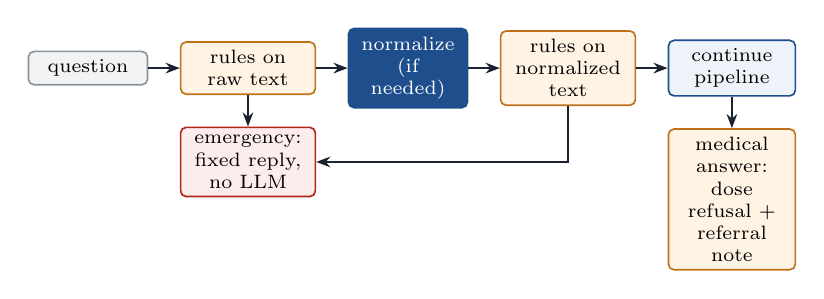
\begin{tikzpicture}[font=\tiny, node distance=3mm and 4mm]
\node[grey, text width=13mm] (q) {question};
\node[safe, right=of q, text width=15mm] (r1) {rules on raw text};
\node[lora, right=of r1, text width=13mm] (n) {normalize (if needed)};
\node[safe, right=of n, text width=15mm] (r2) {rules on normalized text};
\node[box, fill=redlt, draw=redd, below=4mm of r1, text width=15mm] (em) {emergency: fixed reply, no LLM};
\node[box, right=of r2, text width=14mm] (on) {continue pipeline};
\node[safe, below=4mm of on, text width=14mm] (out) {medical answer: dose refusal + referral note};
\draw[arr] (q) -- (r1); \draw[arr] (r1) -- (n); \draw[arr] (n) -- (r2); \draw[arr] (r2) -- (on); \draw[arr] (on) -- (out);
\draw[arr] (r1) -- (em); \draw[arr] (r2.south) |- (em.east);
\end{tikzpicture}}
\caption{Deterministic safety: emergency rules before and after normalization, and the output guard on every medical answer.}
\label{fig:safety}
\end{figure}

\subsection{Dialect Router and Normalization Trigger}
The dialect router classifies a question as Standard, Chittagonian or Sylheti from the union of character $n$-grams (1--5, word-bounded, robust to spelling variation) and word $n$-grams (1--2), weighted by TF-IDF, with a class-balanced linear SVM whose scores are calibrated with 3-fold sigmoid calibration; the regularisation constant $C$ is tuned on DEV macro-F1. Logistic regression, Complement Naive Bayes and single-feature variants are the alternatives, and a fine-tuned BanglaBERT \cite{bhattacharjee2022banglabert} tests whether a transformer router is worth its cost. The normalization trigger is
\begin{equation}
\mathrm{normalize}(q)=\big[v\neq\mathrm{Std}\wedge p_v\ge 0.45\big]\vee\big[q\ \text{is romanized}\big],
\end{equation}
so a Standard question is never rewritten unless the router is at least moderately sure it is dialectal.

\subsection{Normalization Expert}
The normalization expert is a LoRA adapter trained on 24,000 examples drawn from the training pairs in both directions: dialect or romanized $\rightarrow$ Standard (Chittagonian, Sylheti, and romanized input including romanized Standard Bangla) and Standard $\rightarrow$ dialect. The variety is named in the prompt; 15\% of dialect prompts carry a generic ``regional Bangla'' label instead, so the expert also works when the router is unsure. It was trained for one epoch (1,500 steps) and, as a DEV-selected improvement, re-trained for two epochs; the two-epoch expert was adopted because it was better on DEV (78.67 vs.\ 77.24 chrF++). The reverse direction is used only to build the paired test set (Section~\ref{sec:paired}). When the expert's mean token log-probability for a rewrite is below $-0.9$, the system shows its interpretation and asks the user to confirm it.

\textbf{Baselines.} Zero-shot prompting of the base model, and 5-shot prompting whose examples are the five most similar training pairs (character 2--4-gram TF-IDF, same variety and script), a stronger baseline than fixed examples; the BanglaCHQ-Prantik metric set \cite{prantik2025} is reported next to chrF++. A LoRA expert on a 16-bit base with identical data, steps and seed answers the LoRA-vs-QLoRA question.

\subsection{Domain Router}
The domain router uses the same features and classifier over four classes (education, general, medical, other), trained on 6,000 balanced questions per class. It runs on the \emph{normalized} question, so dialect words do not confuse it.

\subsection{Answer / Clarify / Abstain Controller}
The controller decides whether to answer, ask for clarification or abstain from 20 features (Fig.~\ref{fig:controller}). Logistic regression and gradient-boosted trees \cite{friedman2001gbm} are compared with 5-fold cross-validation on DEV (macro-F1). Its data combine clear in-scope questions (ANSWER), out-of-scope sentences (ABSTAIN) and constructed under-specified questions such as a symptom without context (CLARIFY). Abstention because the \emph{evidence} lacks the answer is not the controller's job: the experts learn it from real unanswerable questions.

\begin{figure}[!t]
\centering
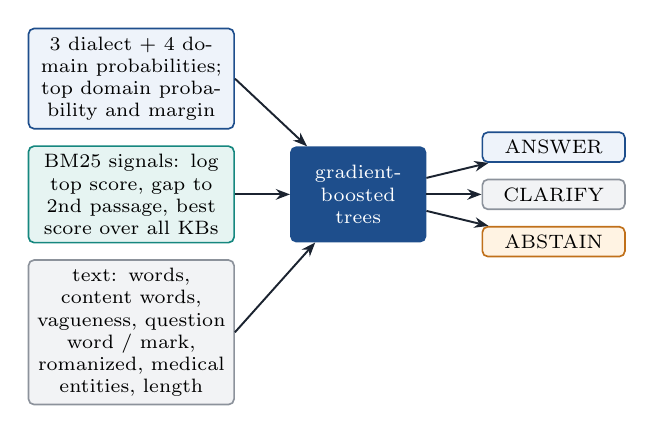
\begin{tikzpicture}[font=\tiny, node distance=2mm]
\node[box, text width=24mm] (f1) {3 dialect + 4 domain probabilities; top domain probability and margin};
\node[cpu, text width=24mm, below=of f1] (f2) {BM25 signals: log top score, gap to 2nd passage, best score over all KBs};
\node[grey, text width=24mm, below=of f2] (f3) {text: words, content words, vagueness, question word / mark, romanized, medical entities, length};
\node[box, fill=navy, text=white, right=7mm of f2, text width=15mm, minimum height=12mm] (gb) {gradient-boosted trees};
\node[box, right=7mm of gb, yshift=6mm, text width=16mm] (a) {ANSWER};
\node[grey, right=7mm of gb, text width=16mm] (c) {CLARIFY};
\node[safe, right=7mm of gb, yshift=-6mm, text width=16mm] (b) {ABSTAIN};
\draw[arr] (f1.east) -- (gb); \draw[arr] (f2) -- (gb); \draw[arr] (f3.east) -- (gb);
\draw[arr] (gb) -- (a); \draw[arr] (gb) -- (c); \draw[arr] (gb) -- (b);
\end{tikzpicture}
\caption{The controller's 20 features and its three decisions.}
\label{fig:controller}
\end{figure}

\subsection{Retrieval per Domain}
Each domain has its own knowledge base. Four retriever families are compared on DEV (Standard questions, document-level nDCG@10): BM25, character TF-IDF, dense retrieval with BGE-M3 or multilingual-E5-base, and hybrids fused by RRF (Eq.~\ref{eq:rrf}). The retriever is chosen \emph{per domain}; a dense method is taken only if it beats the best sparse method by at least 0.01 nDCG@10, because dense search costs GPU time. The result is BM25 for education and general knowledge and dense BGE-M3 for medicine. The expert receives the top $k=3$ passages (at most 600 characters each, 1,800 in total).

\textbf{Dialect-invariant encoder.} As a novel variant, BGE-M3 is fine-tuned so that a dialect sentence $x_i$ and its Standard translation $y_i$ embed close together, with the symmetric InfoNCE loss \cite{oord2018cpc} over a batch of $B=32$ pairs:
\begin{equation}
\mathcal{L}=-\frac{1}{2B}\sum_{i=1}^{B}\Big[\log\frac{e^{s_{ii}/\tau}}{\sum_j e^{s_{ij}/\tau}}+\log\frac{e^{s_{ii}/\tau}}{\sum_j e^{s_{ji}/\tau}}\Big],
\end{equation}
where $s_{ij}=\cos(\mathbf{e}_{x_i},\mathbf{e}_{y_j})$,
$\tau=0.05$, 600 steps and learning rate $2\times10^{-5}$. Every third batch replays (question, gold passage) pairs so that retrieval ability is not forgotten; the encoder is evaluated exactly like the others.

\subsection{Routed Experts and the Pooled Control}
Three answer experts (education, general, medical) are trained on their domain's QA data with three retrieved passages in the prompt (Table~\ref{tab:train}). As a control, one \emph{pooled} adapter is trained on the union of all expert data with the same total number of optimizer steps as all experts together (3,184 steps, 317 vs.\ 316 minutes), so ``routed experts vs.\ one adapter'' is compared at equal compute. Table~\ref{tab:hyper} lists the shared hyper-parameters.

\begin{table}[!t]
\centering
\caption{Adapters trained on Gemma-4-E4B-it (QLoRA unless stated).}
\label{tab:train}
\scriptsize
\begin{tabular}{@{}lrrrr@{}}
\toprule
Adapter & Examples & Steps & Minutes & Peak GB \\
\midrule
Normalization & 24,000 & 1,500 & 72.9 & 19.9 \\
Education & 11,943 & 746 & 112.6 & 30.3 \\
General & 7,994 & 499 & 76.0 & 29.1 \\
Medical (2 epochs) & 3,513 & 439 & 54.9 & 34.7 \\
Pooled (all data) & 47,450 & 3,184 & 316.6 & 34.7 \\
Normalization, LoRA 16-bit & 24,000 & 1,500 & 60.0 & 18.1 \\
\bottomrule
\end{tabular}
\end{table}

\begin{table}[!t]
\centering
\caption{Shared training and decoding settings.}
\label{tab:hyper}
\scriptsize
\begin{tabularx}{\linewidth}{@{}L{2.9cm} Y@{}}
\toprule
Setting & Value \\
\midrule
Base model & Gemma-4-E4B-it, 4-bit NF4, double quantization, BF16 compute \\
LoRA & $r=16$, $\alpha=32$, dropout 0.05, all attention and MLP projections \\
Optimizer & AdamW \cite{loshchilov2019adamw}, learning rate $2\times10^{-4}$, 3\% warm-up, cosine decay \\
Batch & 4 examples $\times$ 4 accumulation steps = 16 \\
Sequence limit & 4,096 tokens (0 examples dropped) \\
Seed & 17 (finalists of S2: 17, 42, 101) \\
Decoding & greedy; 96 new tokens for normalization (up to 384 for long questions), 64 for education/general, 200 for medical \\
Evidence & $k=3$ passages, best first \\
\bottomrule
\end{tabularx}
\end{table}

% =============================================================================
\section{Evaluation Protocol}
\label{sec:eval}

\subsection{Metrics}
\textbf{Normalization} uses chrF++ as the primary metric \cite{popovic2017chrfpp}, because character $n$-grams tolerate the spelling variation typical of dialects:
\begin{equation}
\mathrm{chrF}_\beta=(1+\beta^2)\frac{\mathrm{chrP}\cdot\mathrm{chrR}}{\beta^2\,\mathrm{chrP}+\mathrm{chrR}},\quad\beta=2,
\end{equation}
where chrP and chrR are the character $n$-gram ($n\le6$) precision and recall; chrF++ adds word unigrams and bigrams. BLEU \cite{papineni2002bleu} (computed with sacreBLEU \cite{post2018sacrebleu}), character error rate and, for comparisons with published work, ROUGE \cite{lin2004rouge} and METEOR \cite{banerjee2005meteor} are reported as well.

\textbf{Extractive QA} (education, general) uses exact match and token F1:
\begin{equation}
F1=\frac{2PR}{P+R},\quad P=\frac{|\hat a\cap a|}{|\hat a|},\ R=\frac{|\hat a\cap a|}{|a|},
\end{equation}
over the bags of tokens of the predicted answer $\hat a$ and the gold answer $a$ (maximum over gold answers). \textbf{Medical} answers use chrF++ and ROUGE-L against the doctor's answer, plus the referral rate and the share of answer words found in the evidence. \textbf{Retrieval} uses hit@$k$, MRR@10 and nDCG@10 at document level, and \emph{answer-containment} hit@$k$ (the gold answer string occurs in the top-$k$ passages). \textbf{Routers} use accuracy, macro-F1 and ECE.

The end-to-end \textbf{QA score} of a question is its token F1 (education, general) or chrF++/100 (medical), and 0 when an answerable question is not answered; behaviour is scored separately (answered share, correct abstention on unanswerable and out-of-scope questions, clarification on vague ones). The \textbf{dialect gap} is $g_v=\mathrm{QA}_{\mathrm{Std}}-\mathrm{QA}_v$, and the share of the gap a system closes is
\begin{equation}
\mathrm{closed}_v=\frac{g_v^{\,\mathrm{NO\_NORM}}-g_v^{\,\mathrm{system}}}{g_v^{\,\mathrm{NO\_NORM}}}.
\end{equation}

\subsection{Statistics}
All tables report 95\% percentile-bootstrap confidence intervals over test items \cite{efron1993bootstrap,koehn2004bootstrap}. Two systems evaluated on the same items are compared with a paired approximate-randomization test \cite{riezler2005randomization}: the per-item scores of the two systems are randomly swapped 2,000--5,000 times, and $p$ is the share of swaps whose mean difference is at least as large as the observed one. The full system is compared with seven ablations in three varieties plus the oracle, giving 22 $p$-values, which are corrected with the Holm procedure \cite{holm1979}: with $p_{(1)}\le\dots\le p_{(m)}$, the $i$-th hypothesis is rejected while $p_{(i)}\le\alpha/(m-i+1)$.

\subsection{Paired End-to-End Test Set}
\label{sec:paired}
Dialect QA test data with reference answers do not exist. We therefore take 780 test questions (200 each from education, general and medical, plus 60 unanswerable, 60 out-of-scope and 60 under-specified), rewrite each into Chittagonian and Sylheti with the reverse direction of the normalization expert, and keep a dialect version only if it differs from the original and a round trip back to Standard reaches chrF++ $\ge 40$ (Fig.~\ref{fig:paired}). 92.3\% of the Chittagonian and 92.9\% of the Sylheti versions were kept, giving 2,225 questions: the \emph{same} questions in three varieties, so any score difference is caused by the variety alone.

\begin{figure}[!t]
\centering
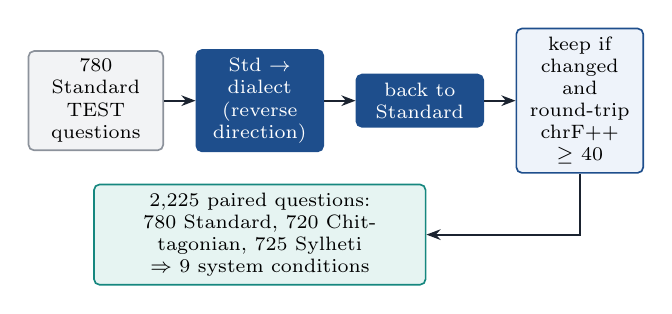
\begin{tikzpicture}[font=\tiny, node distance=3mm and 4mm]
\node[grey, text width=15mm] (s) {780 Standard TEST questions};
\node[lora, right=of s, text width=14mm] (d) {Std $\rightarrow$ dialect (reverse direction)};
\node[lora, right=of d, text width=14mm] (b) {back to Standard};
\node[box, right=of b, text width=14mm] (f) {keep if changed and round-trip chrF++ $\ge$ 40};
\node[cpu, below=4mm of d, text width=40mm] (o) {2,225 paired questions: 780 Standard, 720 Chittagonian, 725 Sylheti $\Rightarrow$ 9 system conditions};
\draw[arr] (s) -- (d); \draw[arr] (d) -- (b); \draw[arr] (b) -- (f); \draw[arr] (f.south) |- (o.east);
\end{tikzpicture}
\caption{Building the paired test set. Because the dialect versions are model-written and ``lighter'' than real dialect text, a second evaluation uses 481 questions written by native speakers (Section~\ref{sec:human}).}
\label{fig:paired}
\end{figure}

\subsection{Human-Written Dialect Questions}
\label{sec:human}
The question sentences in the held-out test split of the native-written parallel corpora (Kothon, Vashantor, ChatgaiyyaAlap, ONUBAD) give 481 real dialect questions (234 Chittagonian, 247 Sylheti), each with its human Standard translation but without a reference answer. The system is therefore evaluated by \emph{consistency}: does it treat the dialect question like its Standard version (same decision, same domain, similar answer, overlapping evidence)?

\subsection{Ablation Conditions}
Table~\ref{tab:conditions} lists the nine conditions run on the paired test set. Each removes or replaces one component, so the difference to \cond{FULL} measures that component's contribution.

\begin{table}[!t]
\centering
\caption{End-to-end evaluation conditions.}
\label{tab:conditions}
\scriptsize
\begin{tabularx}{\linewidth}{@{}L{2.75cm} Y L{1.3cm}@{}}
\toprule
Condition & What is changed & Answers \\
\midrule
\condt{FULL} & nothing (proposed system) & per variety \\
\condt{NO\_NORMALIZATION} & dialect text goes straight to routing, retrieval, expert & RQ2 \\
\condt{ALWAYS\_NORMALIZE} & dialect router bypassed; everything normalized & router value \\
\condt{NO\_DOMAIN\_ROUTING} & one merged KB and the pooled adapter & RQ3 \\
\condt{POOLED\_ADAPTER} & routed experts $\rightarrow$ one pooled adapter & RQ3 \\
\condt{BASE\_MODEL} & no fine-tuning (same prompts) & RQ3 \\
\condt{NO\_RAG} & closed-book answering & RQ3 \\
\condt{NO\_CONTROLLER} & always answer & RQ3 \\
\condt{ORACLE\_STANDARD} & gold Standard question and domain & upper bound \\
\bottomrule
\end{tabularx}
\end{table}

\subsection{Comparability with Published Work}
To compare with published dialect-translation models, the normalization expert is also scored on the \emph{official} Vashantor test sentences \cite{faria2023vashantor} with the papers' own metrics (BLEU, BLEU-1, chrF, METEOR, WER, CER) and 95\% bootstrap intervals; an audit confirms that these sentences are the official test split and never occur in training. The QA experts are compared with the gold-passage results of BanglaRQA and NCTB-QA on the subset of questions whose gold passage was retrieved.

\subsection{Answer-Time Improvements (System v2)}
\label{sec:v2}
After the main results were frozen, a set of improvements that change only \emph{how} the trained models are used was defined (Table~\ref{tab:v2}, Fig.~\ref{fig:v2}). Each was switched on only if it improved the DEV split by a fixed margin (0.005 for retrieval and QA scores). The paired TEST set was then answered once more: a run with every change switched off, on 300 sampled test questions, checks that the v2 code reproduces the reported answers (validity check), and the adopted changes are added one at a time so that each step has its own paired test. The main results stay as reported; v2 is an extension.

The last column of Table~\ref{tab:v2} records the DEV decisions. Three changes were adopted: re-ranking of 50 candidates for education and general questions, with near-duplicate removal for education only (I4); searching both the education and the general knowledge base when the domain router's confidence is below $\tau=0.9$, which happened for about 46\% of DEV questions (I5); and the routing-independent medical note (I3). The other five were tested and not adopted, because they did not reach the DEV margin. The glossary helped Chittagonian but hurt Sylheti. Dual-query retrieval changed answer containment by less than 0.005. A forced second decoding did not raise the DEV QA score for any threshold. Repetition trimming lowered it slightly. The trigger chosen on DEV was the S5 rule itself.

\begin{table}[!t]
\centering
\caption{Answer-time improvements (no retraining), each chosen on DEV.}
\label{tab:v2}
\scriptsize
\begin{tabularx}{\linewidth}{@{}l Y L{2.0cm} L{3.1cm}@{}}
\toprule
& Change & DEV criterion & DEV decision \\
\midrule
I1 & also normalize ``Standard'' predictions with confidence $<t$ & Youden's $J$ \cite{youden1950index} on dialect-ID DEV & not adopted: the S5 rule had the highest $J$ (0.958) \\
I3 & medical note and dose refusal whenever a medical signal fires, independent of routing & F2 on domain DEV & \textbf{adopted}: domain-router medical probability $\ge 0.2$ \\
I4 & 50 candidates, near-duplicate removal \cite{lee2022dedup}, cross-encoder re-ranking \cite{nogueira2019passage,bgereranker2024} & answer-containment hit@3 & \textbf{adopted}: education re-rank + de-duplication (0.730 $\rightarrow$ 0.812); general re-rank (0.727 $\rightarrow$ 0.749) \\
I5 & search education and general KBs when the domain router's confidence $<\tau$ \cite{lee2025routerretriever} & answer-containment hit@3 & \textbf{adopted}: $\tau=0.9$ (0.697 $\rightarrow$ 0.767) \\
I6 & when the expert says ``not found'', decode again with that sentence blocked; keep it if mean log-prob.\ $\ge\theta$ & DEV QA, abstention $-5$ pts max & not adopted: DEV QA unchanged (0.540) at every $\theta$ \\
I7 & cut an answer where it starts repeating itself \cite{xu2022ditto} & DEV QA not lower & not adopted: 0.540 $\rightarrow$ 0.539 \\
I8 & dialect glossary (word entries, TRAIN split) shown to the normalization expert as example turns & chrF++ $\ge$ +0.5, no variety lower & not adopted: Chittagonian $+0.55$, Sylheti $-0.73$ \\
I9 & retrieve with original \emph{and} normalized question, fused by RRF \cite{rackauckas2024ragfusion} & hit@3 on dialectized DEV & not adopted: mean gain $<0.005$ \\
\bottomrule
\end{tabularx}
\end{table}

\begin{figure}[!t]
\centering
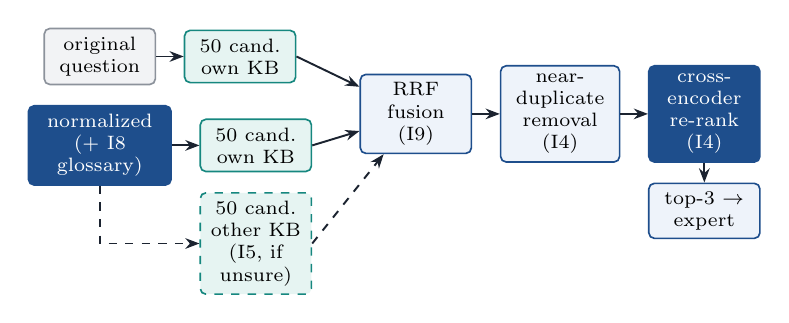
\begin{tikzpicture}[font=\tiny, node distance=2.5mm and 3.5mm]
\node[grey, text width=12mm] (q) {original question};
\node[lora, below=of q, text width=16mm] (n) {normalized (+ I8 glossary)};
\node[cpu, right=of q, text width=12mm] (c1) {50 cand.\ own KB};
\node[cpu, right=of n, text width=12mm] (c2) {50 cand.\ own KB};
\node[cpu, below=of c2, text width=12mm, dashed] (c3) {50 cand.\ other KB (I5, if unsure)};
\node[box, right=6mm of c2, text width=12mm, yshift=4mm] (f) {RRF fusion (I9)};
\node[box, right=of f, text width=13mm] (d) {near-duplicate removal (I4)};
\node[box, fill=navy, text=white, right=of d, text width=12mm] (r) {cross-encoder re-rank (I4)};
\node[box, below=of r, text width=12mm] (t) {top-3 $\rightarrow$ expert};
\draw[arr] (q) -- (c1); \draw[arr] (n) -- (c2); \draw[darr] (n.south) |- (c3.west);
\draw[arr] (c1.east) -- (f); \draw[arr] (c2.east) -- (f); \draw[darr] (c3.east) -- (f);
\draw[arr] (f) -- (d); \draw[arr] (d) -- (r); \draw[arr] (r) -- (t);
\end{tikzpicture}
\caption{Retrieval in system v2 as designed. After the DEV decisions (Table~\ref{tab:v2}), the adopted path is: normalized question $\rightarrow$ 50 candidates from the domain's KB, plus 50 from the other KB when the domain router's confidence is below 0.9 (I5) $\rightarrow$ near-duplicate removal (education) $\rightarrow$ cross-encoder re-ranking $\rightarrow$ top 3. The glossary (I8) and RRF fusion (I9) were tested but not adopted.}
\label{fig:v2}
\end{figure}

% =============================================================================
\section{Implementation Environment}
\label{sec:impl}
The implementation is a Python 3.12 library of 20 modules (data, metrics, retrieval, routers, prompts, training and inference, pipeline, analysis, reporting) embedded in the stage notebooks, so each notebook runs on a fresh machine. The GPU stack is PyTorch 2.8 (CUDA 12.8), Hugging Face Transformers 4.57 (and 5.x in a second environment for Gemma-4), PEFT 0.21, bitsandbytes 0.50 and Accelerate 1.15; the CPU stack adds scikit-learn 1.6 and sacreBLEU 2.5. GPU jobs run detached with atomic checkpoints (adapter, optimizer, scheduler, data order and random states), so a stopped machine resumes where it stopped. Fig.~\ref{fig:gpu} shows the GPU time per stage.

\begin{figure}[!t]
\centering
\resizebox{\linewidth}{!}{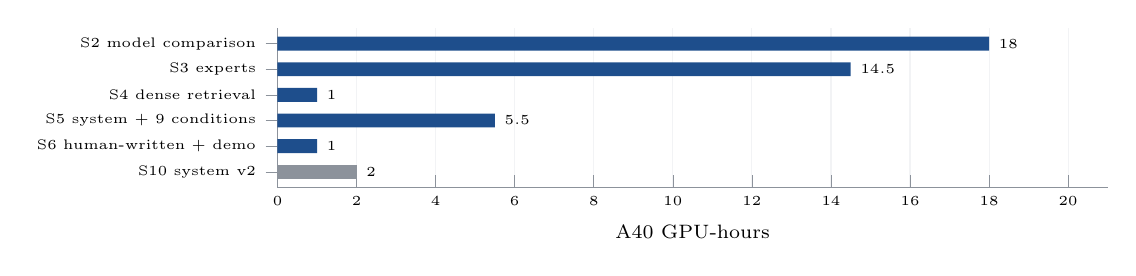
\begin{tikzpicture}
\begin{axis}[width=\linewidth, height=36mm, xbar, bar width=5pt, xmin=0, xmax=21,
  symbolic y coords={S10 system v2,S6 human-written + demo,S5 system + 9 conditions,S4 dense retrieval,S3 experts,S2 model comparison},
  ytick={S10 system v2,S6 human-written + demo,S5 system + 9 conditions,S4 dense retrieval,S3 experts,S2 model comparison}, xlabel={A40 GPU-hours}, nodes near coords, nodes near coords style={font=\tiny}, bar shift=0pt,
  enlarge y limits=0.12, xmajorgrids, ymajorgrids=false]
\addplot[fill=navy, draw=none] coordinates {(18,S2 model comparison) (14.5,S3 experts) (1,S4 dense retrieval) (5.5,S5 system + 9 conditions) (1,S6 human-written + demo)};
\addplot[fill=greyd, draw=none] coordinates {(2,S10 system v2)};
\end{axis}
\end{tikzpicture}}
\caption{GPU time per stage: about 40 A40 GPU-hours ($\approx$US\$20 at US\$0.49/h) up to S6; system v2 added about 2 more hours.}
\label{fig:gpu}
\end{figure}

% =============================================================================
\section{Summary}
The methodology turns a Standard-only QA problem into a dialect-aware one with small, inspectable parts: a CPU dialect router decides \emph{whether} to rewrite, one LoRA expert rewrites, a CPU domain router and controller decide \emph{where} and \emph{whether} to answer, each domain retrieves its own evidence, and one LoRA expert per domain answers from it on a single shared 4-bit model, with deterministic rules for emergencies and medicines. Every decision is made on validation data, every result is reported per language variety, and the evaluation isolates the effect of each component: the same questions in three varieties, nine conditions with Holm-corrected paired tests, native-speaker questions, comparisons with published work on the same test sentences, and a DEV-selected set of answer-time improvements. Chapter~5 reports the results.



\phantomsection
\printbibliography[heading=bibintoc,title={Bibliography}]
\end{document}
